\documentclass[conference]{IEEEtran}
% Compile: pdflatex, bibtex, pdflatex, pdflatex (IEEEtran.cls and IEEEtran.bst required).
\usepackage{cite}
\usepackage{amsmath,amssymb}
\usepackage{graphicx}
\usepackage{textcomp}
\usepackage{array}
\usepackage{booktabs}
\usepackage[hyphens]{url}
\usepackage[T1]{fontenc}

\begin{document}

\title{Thermal-Aware Scheduling for AR/VR-Inspired Workloads: A Reproducible Simulation Study of EDF, a Thermal-Aware EDF Variant and Classical Baselines}

\author{\IEEEauthorblockN{Shreevidha Gour (25BCE1337) \quad Vidhi Gulgulia (25BCE1944) \quad Yahvi Tewari (25BCE5364)}
\IEEEauthorblockA{\textit{B.Tech Computer Science and Engineering, School of Computer Science and Engineering, Vellore Institute of Technology}}}

\maketitle

\begin{abstract}
Augmented- and virtual-reality (AR/VR) applications combine sustained computation with tight timing requirements, so on mobile processors they are exposed to both heat build-up and frequency throttling. This paper asks how scheduling policy, dynamic voltage and frequency scaling (DVFS) and task-migration overhead jointly affect responsiveness and simulated thermal behaviour under AR/VR-inspired workloads. We answer the question with a deterministic, tick-based Python simulator of two identical cores, a first-order thermal model and a threshold DVFS governor. Eight policies are compared: first-come first-served (FCFS), static priority, round robin, the original ThermOS-VR heuristic, non-preemptive and preemptive earliest deadline first (EDF), a thermal-aware EDF variant (TA-EDF) proposed here, and an EEVDF-inspired weighted-fair policy. The main benchmark contains 64 runs over four workloads of six one-shot tasks, and a separate sensitivity study adds 1,024 runs with migration and context-switch costs. Under an identical governor, ThermOS-VR produced exactly the same results as FCFS, which shows that its earlier thermal benefit came from DVFS rather than from its core-scoring rule. The EDF variants gave the lowest or tied-lowest waiting time and total tardiness in every configuration. With free migrations, TA-EDF lowered the simulated peak temperature by 0.08--2.49 \textdegree{}C relative to EDF while matching its responsiveness; once each migration cost 0.1 work units or more, TA-EDF had higher tardiness and a longer makespan than EDF in all 96 matched configurations. All temperatures are model outputs; no hardware, power or energy measurements were made.
\end{abstract}

\begin{IEEEkeywords}
Thermal-aware scheduling, earliest deadline first, dynamic voltage and frequency scaling, AR/VR workloads, task migration, discrete-time simulation, reproducibility
\end{IEEEkeywords}

\section{Introduction}\label{sec:intro}
AR/VR applications run several interacting activities at once: frame rendering, head and hand tracking, physics, sensor fusion and audio. Users perceive delays between head motion and the displayed image, and both perception thresholds and measurement methods for this motion-to-photon latency have been studied in head-mounted displays~\cite{jerald2009,zhao2017}. Delivering high-quality VR on phone-class hardware therefore requires careful use of limited compute resources~\cite{lai2017}. The same workloads heat the device: measurements on smartphones running VR video streaming and an AR game reported steadily rising component and surface temperatures over 20-minute sessions despite frequency scaling, with peak CPU and GPU temperatures above 70 \textdegree{}C in the AR case~\cite{zhang2020}.

Operating systems manage this tension through two complementary mechanisms. Dynamic thermal management and DVFS lower the operating frequency when temperature rises, which reduces power density but also slows execution~\cite{brooks2001,pillai2001}. Scheduling decides \emph{which} task runs \emph{where} and \emph{when}; thermal-aware schedulers additionally use temperature when placing or ordering work~\cite{kong2012}. Whether the scheduler itself can reduce thermal stress without harming responsiveness, or whether frequency control is doing most of the work, is not obvious, and the answer can depend on overheads that simple models ignore.

This study began as an undergraduate operating-systems project, ThermOS-VR, which proposed a scoring heuristic that places each task on the core with the best combination of temperature, core type and deadline urgency. An audit of the original prototype found that its comparison baselines were not equivalent: only some of them used DVFS, and one baseline contained a defect that could run a task on two cores in the same tick. We therefore rebuilt the evaluation around a single shared engine and asked a sharper question: \emph{how do scheduling policy, DVFS and migration overhead jointly affect responsiveness and simulated thermal behaviour under AR/VR-inspired workloads?}

The work is a simulation study. No kernel was modified, no headset or phone was measured, and all temperatures are outputs of an uncalibrated first-order model. Within that scope, the paper makes the following contributions:

\begin{itemize}
\item A verified tick-based simulator in which eight policies share identical workloads, thermal parameters, governor settings and metric definitions, together with tests, independent recomputation of every reported metric and checksum-based preservation of all outputs.
\item Evidence that the original ThermOS-VR score is equivalent to FCFS once both use the same governor, and a correction of an invalid baseline from the earlier prototype.
\item An evaluation of deadline-driven baselines (non-preemptive and preemptive EDF) and of TA-EDF, a thermal-aware EDF variant introduced here, with DVFS disabled and enabled.
\item A 1,024-run sensitivity analysis showing that TA-EDF's parity with EDF depends on migrations being free.
\item A transparent account of negative and null results, including a TA-EDF mechanism that never activated and a fairness property that does not hold on two cores.
\end{itemize}

Section~\ref{sec:related} reviews related work. Section~\ref{sec:model} describes the system model, Section~\ref{sec:policies} the policies and Section~\ref{sec:method} the methodology. Section~\ref{sec:results} presents the results, Section~\ref{sec:discussion} interprets them, Section~\ref{sec:limits} lists limitations and future work, and Section~\ref{sec:conclusion} concludes.

\section{Related Work}\label{sec:related}
\subsection{Deadline-Driven Scheduling}\label{sec:rw-rt}
Liu and Layland analysed fixed-priority and deadline-driven scheduling of periodic tasks on one processor and showed that assigning priorities by the nearest deadline can use the processor fully, which is the basis of EDF~\cite{liu1973}. When preemption is not allowed, feasibility analysis changes; Jeffay, Stanat and Martel studied non-preemptive scheduling of periodic and sporadic tasks and the role of EDF in that setting~\cite{jeffay1991}. Dhall and Liu studied the scheduling of periodic time-critical tasks on multiprocessors and analysed the worst-case behaviour of assignment heuristics~\cite{dhall1978}. Davis and Burns survey the partitioned, global and hybrid multiprocessor approaches that followed, including the reasons why global policies such as EDF lose the optimality they have on a single processor~\cite{davis2011}.

Linux exposes deadline scheduling as SCHED\textsubscript{DEADLINE}, which combines EDF with the Constant Bandwidth Server (CBS) so that each task is isolated within a reserved budget~\cite{abeni1998,lelli2016}. The kernel documentation describes per-task runtime, deadline and period parameters and an admission test on total bandwidth~\cite{kdoc_deadline}. Our EDF policies are much simpler: they order one-shot tasks by absolute deadline, have no bandwidth reservation and no admission control, and continue to run tasks after their deadlines pass.

\subsection{Proportional-Share Scheduling and EEVDF}\label{sec:rw-fair}
Earliest Eligible Virtual Deadline First (EEVDF) allocates processor time in proportion to client weights. Each client accumulates virtual time, is eligible only while it has not received more than its share, and the eligible client with the earliest virtual deadline runs next; for a single resource the deviation from ideal service is bounded by one quantum~\cite{stoica1995}. Proportional fairness is harder to guarantee on several processors: Pfair scheduling formalises proportionate progress on multiprocessors~\cite{baruah1996}, and Chandra \emph{et al.} showed that weights which cannot be honoured on a symmetric multiprocessor lead to unfairness unless they are readjusted~\cite{chandra2000}. Linux adopted a version of EEVDF proposed in 2023~\cite{corbet2023}; its documentation states that the transition began in kernel 6.6 and describes lag, virtual deadlines, requested time slices and deferred dequeue of sleeping tasks~\cite{kdoc_eevdf}. Our EEVDF-inspired policy reproduces the core selection rule but not these kernel mechanisms.

\subsection{Thermal Management and Thermal-Aware Scheduling}\label{sec:rw-thermal}
Brooks and Martonosi argued that dynamic thermal management lets a processor be designed for typical rather than worst-case power, with little performance loss in common workloads~\cite{brooks2001}. Skadron \emph{et al.} introduced temperature-aware microarchitecture and the HotSpot model, and later work presented HotSpot as a compact resistance--capacitance thermal modelling methodology for early design stages~\cite{skadron2003,huang2006}. Kong, Chung and Skadron survey thermal management techniques, including operating-system and compiler approaches~\cite{kong2012}. Real-time DVFS was integrated with scheduling by Pillai and Shin, who showed that voltage scaling must respect deadline guarantees~\cite{pillai2001}.

Thermal-aware scheduling has been studied from several directions. Hung \emph{et al.} proposed thermal-aware task allocation and scheduling for embedded systems~\cite{hung2005}; Coskun, Rosing and Whisnant evaluated operating-system-level temperature-aware scheduling policies for multiprocessor systems-on-chip~\cite{coskun2007}; and Chrobak \emph{et al.} analysed temperature-aware scheduling algorithmically, including online competitiveness results~\cite{chrobak2008}. More recent work combines prediction with DVFS: P\'{e}rez Rodr\'{i}guez and Meumeu Yomsi propose a proactive scheduler for a single DVFS-capable core~\cite{perez2021}, Lee, Shin and Chwa schedule real-time tasks on integrated CPU--GPU platforms while balancing heat (RT-TAS)~\cite{lee2019}, and Dowling \emph{et al.} drive a multi-core thermal-aware scheduler, POD-TAS, with a reduced-order learned thermal model and compare it with RT-TAS in a simulation pipeline~\cite{dowling2025}. These studies use far more detailed thermal models than ours; our contribution is not a better thermal model but a controlled comparison of scheduling policies under one shared, simple model.

\subsection{Heterogeneous and Mobile Platforms}\label{sec:rw-hetero}
Single-ISA heterogeneous multi-core designs run each application on the core that best matches its performance and power needs~\cite{kumar2003}. Linux describes such systems as having asymmetric CPU capacity~\cite{kdoc_capacity}, and its Energy Aware Scheduling (EAS) selects an energy-efficient CPU at task wake-up using an energy model; EAS requires an asymmetric topology, power cost tables and the schedutil governor~\cite{kdoc_eas}. On phones, frequency control has been managed jointly for the CPU and GPU to reduce the power of 3D games~\cite{pathania2014}, and reinforcement learning has been used to trade UI smoothness against power on a commercial Android device~\cite{dou2025}. Detailed smartphone thermal simulators produce chip and skin temperature maps~\cite{xie2014}. Our simulator has two identical cores and no energy model, so it cannot evaluate capacity- or energy-aware placement; we state this limitation explicitly rather than approximating EAS.

\subsection{AR/VR Systems and Evaluation Practice}\label{sec:rw-xr}
ILLIXR provides an open end-to-end XR system for studying real pipelines and their resource demands~\cite{huzaifa2021}; trace-driven workloads of this kind are a natural next step beyond our hand-specified task sets. On methodology, Jain's text covers simulation and performance analysis~\cite{jain1991}, while Georges \emph{et al.} and Hoefler and Belli argue that performance claims require repeated measurements and statistically sound reporting~\cite{georges2007,hoefler2015}. Because our simulator is deterministic and each configuration was executed once, we report observed differences without significance claims. Finally, context switches have measurable indirect costs, mainly through cache interference~\cite{li2007}, which motivates our sensitivity study of migration and context-switch overheads.

\section{System Model and Architecture}\label{sec:model}
Fig.~\ref{fig:arch} shows the simulator. A workload is a set of one-shot tasks. At every tick the engine forms the ready set, asks the active policy for a task-to-core mapping, executes one tick on each core, updates each core's temperature, lets the DVFS governor choose the frequency for the next tick, records completions and logs one trace row per core. The same engine, thermal model, governor and metric code are used for every policy.

\begin{figure}[!t]
\centering
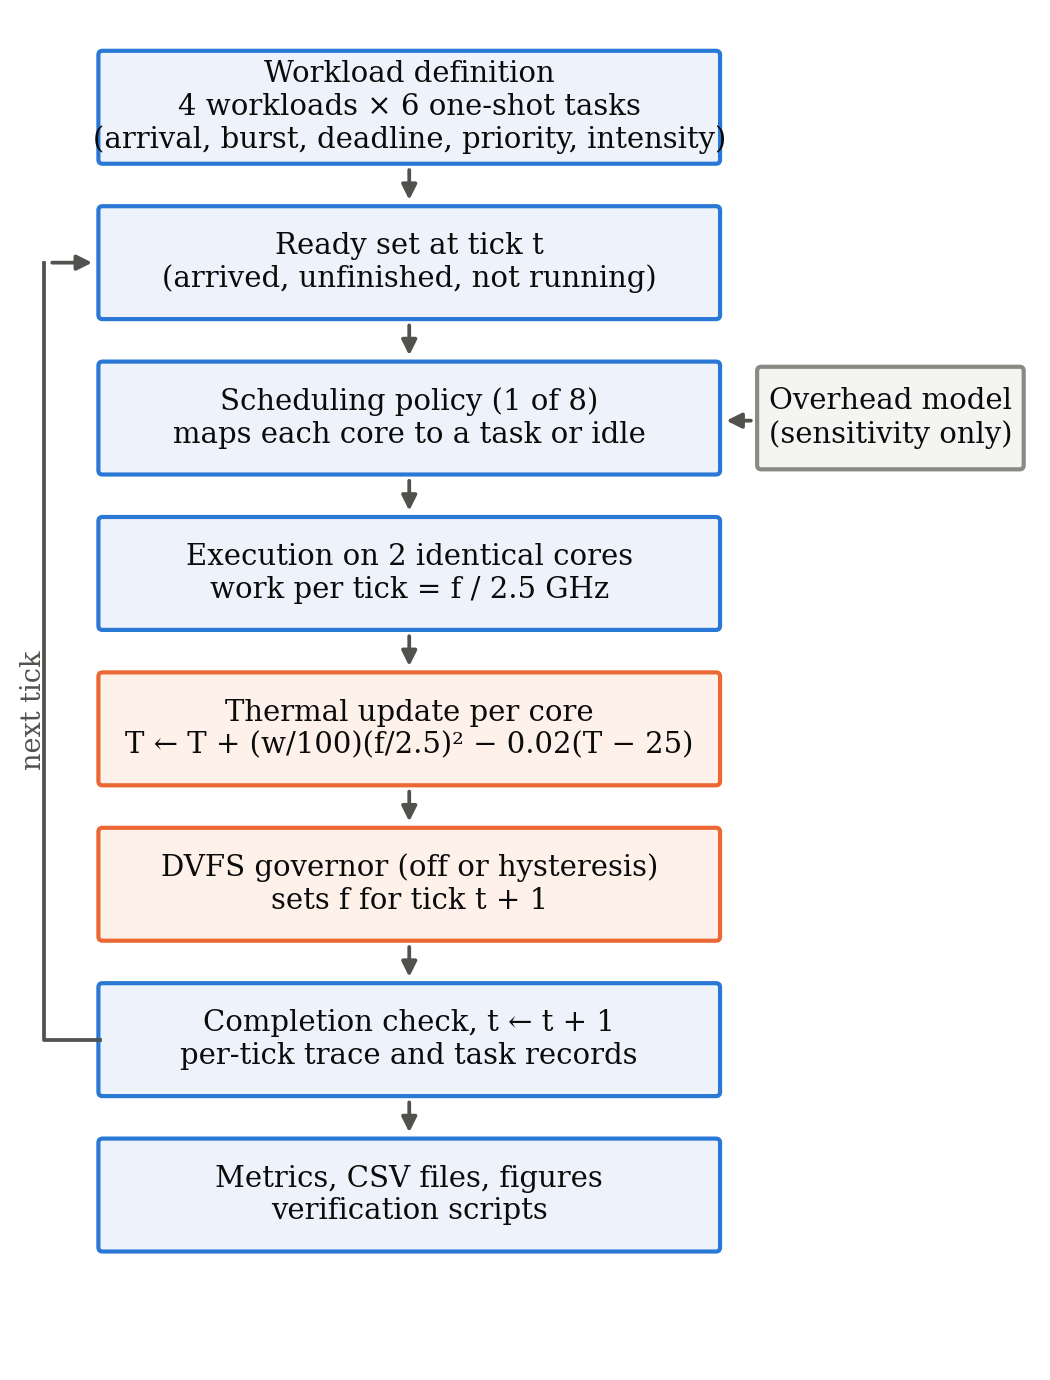
\includegraphics[width=\columnwidth]{figures/fig_architecture.png}
\caption{Simulator architecture and per-tick order. The same engine, thermal model, DVFS governor and metrics are used for all eight policies; the overhead model is used only in the sensitivity experiment.}
\label{fig:arch}
\end{figure}

\subsection{Tasks, Cores and Time}\label{sec:model-tasks}
Each task \emph{i} has an arrival time \emph{a}\textsubscript{i}, a burst (work) \emph{b}\textsubscript{i}, an absolute deadline \emph{d}\textsubscript{i}, a priority and a workload intensity \emph{w}\textsubscript{i} (in percent). Time advances in abstract ticks; the tick has no defined wall-clock length, so no result is converted to milliseconds. The platform has two cores that the original prototype labelled ``Performance'' and ``Efficiency''. In the model the two cores are identical: they have the same frequency levels, the same speed and the same thermal parameters, and no heat flows between them. The labels therefore do not represent hardware heterogeneity.

A core running at frequency \emph{f} completes \emph{f}/2.5 GHz work units per tick, so a task progresses one unit per tick at 2.5 GHz and 0.88 units at 2.2 GHz. Preemption and migration can occur only at tick boundaries. A task finishes at the end of the tick in which its remaining work reaches zero; if that happens partway through a throttled tick, the unused fraction of the tick is still counted as busy time and still generates heat. In the benchmark, 88 of the 384 task records finish partway through their final tick, with at most 0.96 units of unused capacity. This accounting rule is applied identically to every policy, but it slightly overstates busy time and heat.

\subsection{Thermal Model}\label{sec:model-thermal}
Each core's temperature \emph{T} (in model degrees Celsius) evolves by a first-order heating-and-cooling update:

\begin{equation}
T_{k+1} = T_k + \alpha\,\frac{w}{100}\left(\frac{f}{f_{\mathrm{ref}}}\right)^{2} - \beta\,(T_k - T_{\mathrm{amb}})
\label{eq:thermal}
\end{equation}

with $\alpha$ = 1, $\beta$ = 0.02, \emph{f}\textsubscript{ref} = 2.5 GHz and ambient temperature \emph{T}\textsubscript{amb} = 25 \textdegree{}C; every core starts at 45 \textdegree{}C, and an idle core generates no heat (\emph{w} = 0). Thermal states are COOL below 60 \textdegree{}C, WARM below 70 \textdegree{}C, HOT below 80 \textdegree{}C and CRITICAL at or above 80 \textdegree{}C. Under a constant load the temperature converges to

\begin{equation}
T^{*} = T_{\mathrm{amb}} + \frac{\alpha}{\beta}\,\frac{w}{100}\left(\frac{f}{f_{\mathrm{ref}}}\right)^{2},
\label{eq:steady}
\end{equation}

which is 75.0 \textdegree{}C for a fully loaded core at 2.5 GHz and 63.7 \textdegree{}C at 2.2 GHz. The model is linear in temperature and both cores are identical, a property that matters when interpreting placement effects (Section~\ref{sec:discussion}). It is a teaching-scale model: it is not calibrated against any processor, and its outputs are not physical temperatures, powers or energies.

\subsection{DVFS Governor}\label{sec:model-dvfs}
Two DVFS settings are evaluated for every policy. With DVFS \emph{off}, both cores always run at 2.5 GHz. With the \emph{hysteresis} governor, each core steps down one frequency level (2.5 $\rightarrow$ 2.2 $\rightarrow$ 1.8 $\rightarrow$ 1.4 GHz) when its temperature reaches 60, 70 or 80 \textdegree{}C respectively, and steps back up only after cooling to 58, 68 or 78 \textdegree{}C; at most one step is taken per tick. Because a fully loaded core settles at 63.7 \textdegree{}C at 2.2 GHz, only the 2.5 and 2.2 GHz levels occur on the tested workloads; the lower levels were exercised only in a stress test with a higher heat coefficient. Table~\ref{tab:params} summarises the parameters.

\begin{table}[!t]
\centering
\footnotesize
\caption{Simulation parameters (from run metadata and source code)}
\label{tab:params}
\setlength{\tabcolsep}{3pt}
\begin{tabular}{ll}
\toprule
Parameter & Value \\
\midrule
Cores & 2, identical (labels only) \\
Initial / ambient temperature & 45 \textdegree{}C / 25 \textdegree{}C \\
Heat per busy tick & $\alpha$(w/100)(f/2.5)\textsuperscript{2}, $\alpha$ = 1 \\
Cooling per tick & $\beta$(T $-$ 25), $\beta$ = 0.02 \\
Thermal states & COOL < 60, WARM < 70, HOT < 80 \textdegree{}C \\
Frequency levels & 2.5, 2.2, 1.8, 1.4 GHz \\
Work per tick & f / 2.5 GHz units \\
Governor down / up & 60, 70, 80 / 58, 68, 78 \textdegree{}C \\
DVFS settings & off (2.5 GHz), hysteresis \\
TA-EDF rules & urgent s $\leq$ 2; hold-back T $\geq$ 59 \textdegree{}C, s $\geq$ 10 \\
EEVDF slice / weights & 1 tick; 9548, 3121, 1024, 335, 110 \\
Overhead costs (sensitivity) & \{0, 0.1, 0.25, 0.5\} work units \\
Runs & 64 benchmark; 1,024 sensitivity \\
\bottomrule
\end{tabular}
\end{table}

\section{Scheduling Policies}\label{sec:policies}
At each tick a policy receives the ready tasks (arrived, unfinished and not running) and the current cores, and returns the task for each core. A policy preempts a task by not mapping it. Unless stated otherwise, ties are broken by earlier arrival and then lower task identifier, and ``lowest free core'' means the free core with the smaller index. Late tasks are never dropped: every task runs to completion, which corresponds to a soft real-time interpretation. Table~\ref{tab:policies} summarises the eight policies.

\begin{table*}[!t]
\centering
\scriptsize
\caption{Scheduling policies evaluated. Ties: earlier arrival, then lower task identifier. Late tasks are never dropped.}
\label{tab:policies}
\setlength{\tabcolsep}{3pt}
\begin{tabular}{llllll}
\toprule
Policy & Task order & Preemptive & Core choice & Deadline & Temperature \\
\midrule
FCFS & arrival & no & lowest free core & no & no \\
Priority & priority, arrival & no & lowest free core & no & no \\
Round Robin & FIFO queue, quantum 1 & yes & lowest free core & no & no \\
ThermOS-VR & arrival & no & max. score S (3) & constant term & yes \\
EDF-NP & absolute deadline & no & lowest free core & yes & no \\
EDF & absolute deadline & yes & keep core, else lowest free & yes & no \\
TA-EDF (ours) & absolute deadline & yes & urgent: fastest; else coolest & yes (slack) & yes \\
EEVDF-inspired & eligible, virtual deadline & yes & keep core, else lowest free & no & no \\
\bottomrule
\end{tabular}
\end{table*}

\subsection{Classical Baselines}\label{sec:pol-classic}
\emph{FCFS} orders ready tasks by arrival and runs each to completion on the lowest free core. \emph{Priority} is identical except that it orders by static priority (a lower number means higher priority). \emph{Round Robin} (RR) keeps a single first-in first-out queue with a quantum of one tick: at each boundary the tasks whose quantum expired re-enter the queue before newly arrived tasks, and idle cores take tasks from the head of the queue.

\subsection{ThermOS-VR}\label{sec:pol-thermos}
ThermOS-VR keeps FCFS order and non-preemptive execution, but chooses among idle, non-CRITICAL cores by maximising a score

\begin{equation}
S(i,c,t) = 1.5\,(100 - T_c) - \pi(c) + \kappa(i,c) + \delta(i,t),
\label{eq:score}
\end{equation}

where $\pi$(\emph{c}) is a penalty of 10 for a WARM core and 50 for a HOT core, $\kappa$(\emph{i},\emph{c}) favours the ``Performance'' label for intensities of at least 70 \% and the ``Efficiency'' label for intensities of at most 40 \%, and $\delta$(\emph{i},\emph{t}) is 30 if the time to the deadline does not exceed the remaining work and 15 otherwise. The deadline term depends only on the task and the time, not on the core, so it adds the same constant to every candidate and cannot change the ranking. Because the two cores are physically identical and the task order is fixed by FCFS, the remaining terms can change \emph{which} identical core receives a task but not when any task runs. We use a faithful port of the original code; it selects the same core as the original function in 2,000 randomised states.

\subsection{EDF Variants}\label{sec:pol-edf}
\emph{Non-preemptive EDF (EDF-NP)} orders ready tasks by absolute deadline and runs each dispatched task to completion on the lowest free core. \emph{Preemptive global EDF (EDF)} re-selects, at every tick boundary, the two tasks with the earliest deadlines among running and ready tasks; a selected task that is already running keeps its core, and a newly selected task takes the lowest free core, so EDF is thermally blind. Late tasks keep their original deadlines and therefore retain high priority, as in standard EDF.

\subsection{Thermal-Aware EDF (TA-EDF)}\label{sec:pol-taedf}
TA-EDF is the variant proposed in this work; it is not an established scheduler. It uses the same task order as EDF and adds two thermal rules based on the slack

\begin{equation}
s_i(t) = d_i - t - r_i,
\label{eq:slack}
\end{equation}

where \emph{r}\textsubscript{i} is the remaining work. A task is \emph{urgent} if \emph{s}\textsubscript{i} $\leq$ 2. An urgent task takes the free core with the highest current frequency (then the cooler one); any other task takes the coolest free core (then the higher frequency); remaining ties prefer the core the task last ran on. The second rule is a hold-back, or idle-insertion, rule: a task with \emph{s}\textsubscript{i} $\geq$ 10 is skipped for the current tick if its chosen core is at or above 59 \textdegree{}C, one degree below the governor's first threshold, so that the core can cool. A skipped task's slack falls by one per tick, so the delay is bounded. The parameters (2, 59 \textdegree{}C, 10) were fixed before the benchmark and were not tuned. With DVFS off both cores always run at the same frequency, so both placement rules reduce to choosing the coolest free core.

\subsection{EEVDF-Inspired Weighted-Fair Policy}\label{sec:pol-eevdf}
This policy models the defining EEVDF rules~\cite{stoica1995} at tick granularity. Task priorities 1--5 are mapped, by our own assumption, to nice values $-$10, $-$5, 0, 5 and 10 and hence to weights 9548, 3121, 1024, 335 and 110. A task that runs for a tick advances its virtual runtime by 1024/\emph{w}\textsubscript{i}. The policy computes

\begin{equation}
V = \frac{\sum_j w_j v_j}{\sum_j w_j}, \quad \ell_i = w_i (V - v_i), \quad \hat{d}_i = v_i + q\,\frac{1024}{w_i},
\label{eq:eevdf}
\end{equation}

where \emph{V} is the weighted average virtual runtime of runnable tasks, $\ell$\textsubscript{i} is the lag and the virtual deadline is renewed after each slice \emph{q} = 1 tick. A task is eligible when its lag is non-negative, and the eligible tasks with the earliest virtual deadlines run; new tasks start with zero lag. The policy ignores real deadlines and temperatures. It differs from Linux EEVDF in important ways: it uses one global queue rather than per-CPU queues with load balancing, it does not model sleeping, lag decay or wake-up preemption, and, to keep both cores busy, it dispatches an ineligible task when fewer eligible tasks than cores exist. We therefore call it \emph{EEVDF-inspired} and make no claim of Linux-equivalent fairness.

\subsection{Mechanisms Not Evaluated}\label{sec:pol-eas}
Energy Aware Scheduling was not implemented or benchmarked. The kernel documentation states that EAS does not support symmetric CPU topologies and requires an energy model and the schedutil governor~\cite{kdoc_eas}; our two identical cores and the absence of a power model would reduce any EAS-style policy to an arbitrary choice. Likewise, none of the policies is SCHED\textsubscript{DEADLINE}~\cite{kdoc_deadline} or kernel EEVDF~\cite{kdoc_eevdf}.

\section{Experimental Methodology}\label{sec:method}
\subsection{Workloads}\label{sec:method-workloads}
Four workloads inherited from the original prototype are used without modification (Table~\ref{tab:workloads}). Each contains six one-shot tasks named after AR/VR subsystems, with hand-specified arrivals, bursts, deadlines, priorities and intensities. They are AR/VR-\emph{inspired}: they are not traces of real applications and they are not periodic frame tasks. Dividing the total work by two gives a lower bound on the makespan of any two-core schedule at full speed. Normal VR is feasible in aggregate, but Burst VR (total work 63, bound 31.5, deadlines 10--24), Sustained Thermal (245, 122.5, deadlines 45--60) and HOT Thermal (405, 202.5, deadlines 75--100) cannot meet most deadlines under any policy. Deadline-miss counts therefore saturate, and we also report total tardiness, which continues to separate the policies.

\begin{table*}[!t]
\centering
\scriptsize
\caption{Workloads: six one-shot tasks each (times in ticks, intensity in \%). The bound is total work divided by two cores at full speed.}
\label{tab:workloads}
\setlength{\tabcolsep}{3pt}
\begin{tabular}{lllrrrrr}
\toprule
Workload & ID & Task & Arr. & Burst & Deadline & Prio. & Int. \\
\midrule
Normal & 1 & Frame Rendering & 0 & 8 & 10 & 1 & 90 \\
 & 2 & Motion Tracking & 1 & 4 & 8 & 2 & 70 \\
 & 3 & Physics Engine & 2 & 6 & 12 & 3 & 80 \\
 & 4 & Sensor Processing & 3 & 3 & 10 & 2 & 60 \\
 & 5 & Audio & 4 & 2 & 12 & 4 & 30 \\
 & 6 & Background & 5 & 5 & 20 & 5 & 20 \\
 & & \multicolumn{6}{l}{\emph{Total work 28; two-core bound 14}} \\
\midrule
Burst & 1 & Initial Rendering & 0 & 8 & 10 & 1 & 95 \\
 & 2 & Initial Physics & 0 & 8 & 12 & 2 & 90 \\
 & 3 & Burst Rendering & 8 & 15 & 22 & 1 & 100 \\
 & 4 & Burst Physics & 8 & 14 & 24 & 2 & 95 \\
 & 5 & Motion Tracking & 9 & 10 & 20 & 1 & 85 \\
 & 6 & Sensor Burst & 10 & 8 & 21 & 2 & 80 \\
 & & \multicolumn{6}{l}{\emph{Total work 63; two-core bound 31.5}} \\
\midrule
Sustained & 1 & Sustained Rendering & 0 & 50 & 55 & 1 & 100 \\
 & 2 & Sustained Physics & 0 & 50 & 58 & 2 & 95 \\
 & 3 & Continuous Tracking & 0 & 45 & 55 & 1 & 90 \\
 & 4 & Continuous Sensor Processing & 0 & 40 & 55 & 2 & 85 \\
 & 5 & Audio Processing & 5 & 30 & 45 & 3 & 60 \\
 & 6 & Background Compute & 10 & 30 & 60 & 5 & 50 \\
 & & \multicolumn{6}{l}{\emph{Total work 245; two-core bound 122.5}} \\
\midrule
HOT & 1 & Extreme Rendering & 0 & 80 & 90 & 1 & 100 \\
 & 2 & Extreme Physics & 0 & 80 & 95 & 1 & 100 \\
 & 3 & Continuous Tracking & 0 & 75 & 90 & 1 & 95 \\
 & 4 & Heavy Sensor Processing & 0 & 70 & 90 & 2 & 90 \\
 & 5 & Audio Processing & 10 & 50 & 75 & 3 & 70 \\
 & 6 & Background Compute & 20 & 50 & 100 & 5 & 60 \\
 & & \multicolumn{6}{l}{\emph{Total work 405; two-core bound 202.5}} \\
\bottomrule
\end{tabular}
\end{table*}

\subsection{Experimental Design and Metrics}\label{sec:method-design}
The main benchmark runs every combination of eight policies, four workloads and two DVFS settings once, giving 64 runs and 384 task records. Each run uses fresh task and core objects, the same initial temperature and the same metric code. Migration and context-switch costs are zero in this benchmark; their effect is studied separately. The metrics are defined identically for every policy. \emph{Waiting time} counts every tick a task has arrived, is unfinished and is not running, including time after preemption. \emph{Tardiness} is max(0, completion $-$ deadline), summed over tasks, and a deadline is missed when the completion time exceeds it. \emph{Peak} and \emph{average temperature} are taken over all post-tick core samples. \emph{HOT core-ticks} count samples at or above 70 \textdegree{}C, and \emph{core-ticks $\geq$ 60 \textdegree{}C} count samples at or above the governor's first threshold. \emph{Throttled busy core-ticks} count busy samples executed below 2.5 GHz, \emph{heat generated} sums the model's heat term, and a \emph{migration} is counted whenever a task executes on a different core from the one it last executed on.

\subsection{Overhead Sensitivity Experiment}\label{sec:method-overhead}
The second experiment repeats all 64 configurations for every combination of a migration cost and a context-switch cost in \{0, 0.1, 0.25, 0.5\} simulated work units, one unit being one tick of work at 2.5 GHz, which yields 1,024 runs. A dispatch event occurs when a task runs in a tick but did not run on the same core in the previous tick. A first dispatch is free; a dispatch to a different core from the last one is charged the migration cost; a dispatch back to the same core after a gap is charged the context-switch cost. Each event is charged once, so a migration is never also charged as a context switch. The charge is added to the task's remaining work, so the core spends that capacity, and generates the corresponding heat, before the task progresses. The costs are hypothetical fractions of a tick; they are not calibrated to measured latencies, although real context switches do have measurable indirect costs~\cite{li2007}.

\subsection{Corrections, Verification and Reproducibility}\label{sec:method-verify}
The earlier prototype's results were not reused as baselines. Its Thermal-DVFS baseline could assign a running task to a second core in the same tick, its DVFS logic never stepped below 2.2 GHz, its schedulers used different logging rules, and only two of its five schedulers used DVFS. In the new engine, the earlier ``Thermal-DVFS'' baseline is simply FCFS under the hysteresis governor, a runtime check rejects any mapping that places a task on two cores, and all policies share one logging rule. For FCFS, Priority, RR and ThermOS-VR, the engine reproduces the earlier prototype's per-task outcomes and per-tick temperatures exactly when configured with the same governor behaviour.

Table~\ref{tab:verify} lists the verification performed. All checks were executed on the final code and outputs, and every number in this paper was recomputed from the result files by an independent script. The commands to reproduce the experiments are \texttt{python -B run\_benchmark.py}, \texttt{python -B run\_sensitivity.py} and \texttt{python -B plot\_results.py}, followed by \texttt{python -B verify\_outputs.py} and \texttt{python -B verify\_sensitivity.py}; the runners refuse to overwrite existing outputs unless \texttt{--overwrite} is given. The software environment was Python 3.14.0, pandas 3.0.5, matplotlib 3.10.7 and NumPy 2.3.4 on Windows 11.

\begin{table}[!t]
\centering
\footnotesize
\caption{Verification performed on the final code and outputs}
\label{tab:verify}
\setlength{\tabcolsep}{3pt}
\begin{tabular}{>{\raggedright\arraybackslash}p{0.43\columnwidth}>{\raggedright\arraybackslash}p{0.49\columnwidth}}
\toprule
Check & Result \\
\midrule
Unit tests (python -B -m unittest) & 42 tests, OK \\
Metrics recomputed from raw traces & 1,024 values, all equal \\
Fresh re-runs & 64 + 1,024 runs, identical \\
Figures vs CSV & 768 plotted values; 25/25 PNGs pixel-identical \\
EDF vs independent reference & 18,024 comparisons, 0 mismatches \\
v1 equivalence (4 policies) & exact task outcomes and temperatures \\
Zero-overhead sensitivity rows & equal benchmark (64 $\times$ 16 metrics) \\
Numbers quoted in this paper & asserted against the CSVs at build \\
Preservation & 179 frozen files, SHA-256 unchanged \\
\bottomrule
\end{tabular}
\end{table}

\section{Results}\label{sec:results}
All values below come from single deterministic runs. Differences are reported as observed; no statistical significance is implied.

\subsection{ThermOS-VR Versus FCFS}\label{sec:res-thermos}
Under the same governor, ThermOS-VR and FCFS produced identical values for all 16 metrics in all eight workload and DVFS configurations (128 comparisons, none different). Per-core placement differed in Normal VR, where two tasks were placed on the opposite cores, but the cores are identical and the differences cancelled in every metric. The thermal improvement attributed to ThermOS-VR in the earlier prototype is therefore explained by DVFS: for FCFS on the HOT workload, enabling the governor lowered the simulated peak from 71.74 to 62.49 \textdegree{}C and the HOT core-ticks from 64 to 0, while the makespan grew from 205 to 226 ticks. On Sustained Thermal the peak fell from 67.61 to 61.28 \textdegree{}C and the makespan grew from 125 to 135 ticks. Normal VR and Burst VR never reach 60 \textdegree{}C, so the governor does not change them.

\subsection{Responsiveness}\label{sec:res-resp}
Table~\ref{tab:resp} and Fig.~\ref{fig:wait} report the responsiveness metrics with DVFS enabled. An EDF variant attained the minimum waiting time and the minimum total tardiness in all 16 combinations of DVFS setting, workload and metric, often with ties. In Normal VR, a waiting time of 2.83 ticks is shared by Priority, EDF-NP, EDF and TA-EDF, and a total tardiness of 2 ticks is shared by six policies. With DVFS enabled, TA-EDF had the lowest waiting time in Sustained Thermal (40.83 ticks versus 41.33 for EDF) and HOT Thermal (69.17 versus 69.50), while EDF had the lowest tardiness in HOT Thermal (368 versus 369). Across all eight configurations, EDF and TA-EDF never differed by more than 0.5 ticks of waiting time or 2 ticks of tardiness, in both directions; we therefore do not claim that either is more responsive.

\begin{table*}[!t]
\centering
\scriptsize
\caption{Responsiveness with DVFS enabled: average waiting time W and total tardiness T (ticks), and deadline misses M (of 6). Bold marks the minimum, including ties.}
\label{tab:resp}
\setlength{\tabcolsep}{3pt}
\begin{tabular}{lrrrrrrrrrrrr}
\toprule
Policy & \multicolumn{3}{c}{Normal} & \multicolumn{3}{c}{Burst} & \multicolumn{3}{c}{Sustained} & \multicolumn{3}{c}{HOT} \\
\cmidrule(lr){2-4} \cmidrule(lr){5-7} \cmidrule(lr){8-10} \cmidrule(lr){11-13}
 & W & T & M & W & T & M & W & T & M & W & T & M \\
\midrule
FCFS & 3.50 & \textbf{2} & 2 & 4.33 & 23 & 3 & 48.83 & 253 & \textbf{4} & 80.67 & 431 & \textbf{4} \\
Priority & \textbf{2.83} & \textbf{2} & \textbf{1} & 4.33 & 23 & 3 & 47.33 & 247 & \textbf{4} & 80.67 & 431 & \textbf{4} \\
RR & 4.33 & 5 & 2 & 5.83 & 30 & 4 & 71.67 & 378 & 6 & 126.50 & 697 & 6 \\
ThermOS-VR & 3.50 & \textbf{2} & 2 & 4.33 & 23 & 3 & 48.83 & 253 & \textbf{4} & 80.67 & 431 & \textbf{4} \\
EDF-NP & \textbf{2.83} & \textbf{2} & \textbf{1} & 4.33 & 23 & 3 & 42.83 & 217 & \textbf{4} & 72.83 & 383 & \textbf{4} \\
EDF & \textbf{2.83} & \textbf{2} & \textbf{1} & \textbf{3.00} & \textbf{17} & \textbf{2} & 41.33 & 210 & \textbf{4} & 69.50 & \textbf{368} & \textbf{4} \\
TA-EDF & \textbf{2.83} & \textbf{2} & \textbf{1} & \textbf{3.00} & \textbf{17} & \textbf{2} & \textbf{40.83} & \textbf{208} & \textbf{4} & \textbf{69.17} & 369 & \textbf{4} \\
EEVDF-insp. & 3.83 & 3 & 2 & 4.83 & 24 & 4 & 56.50 & 292 & 6 & 101.50 & 542 & 6 \\
\bottomrule
\end{tabular}
\end{table*}

\begin{figure*}[!t]
\centering
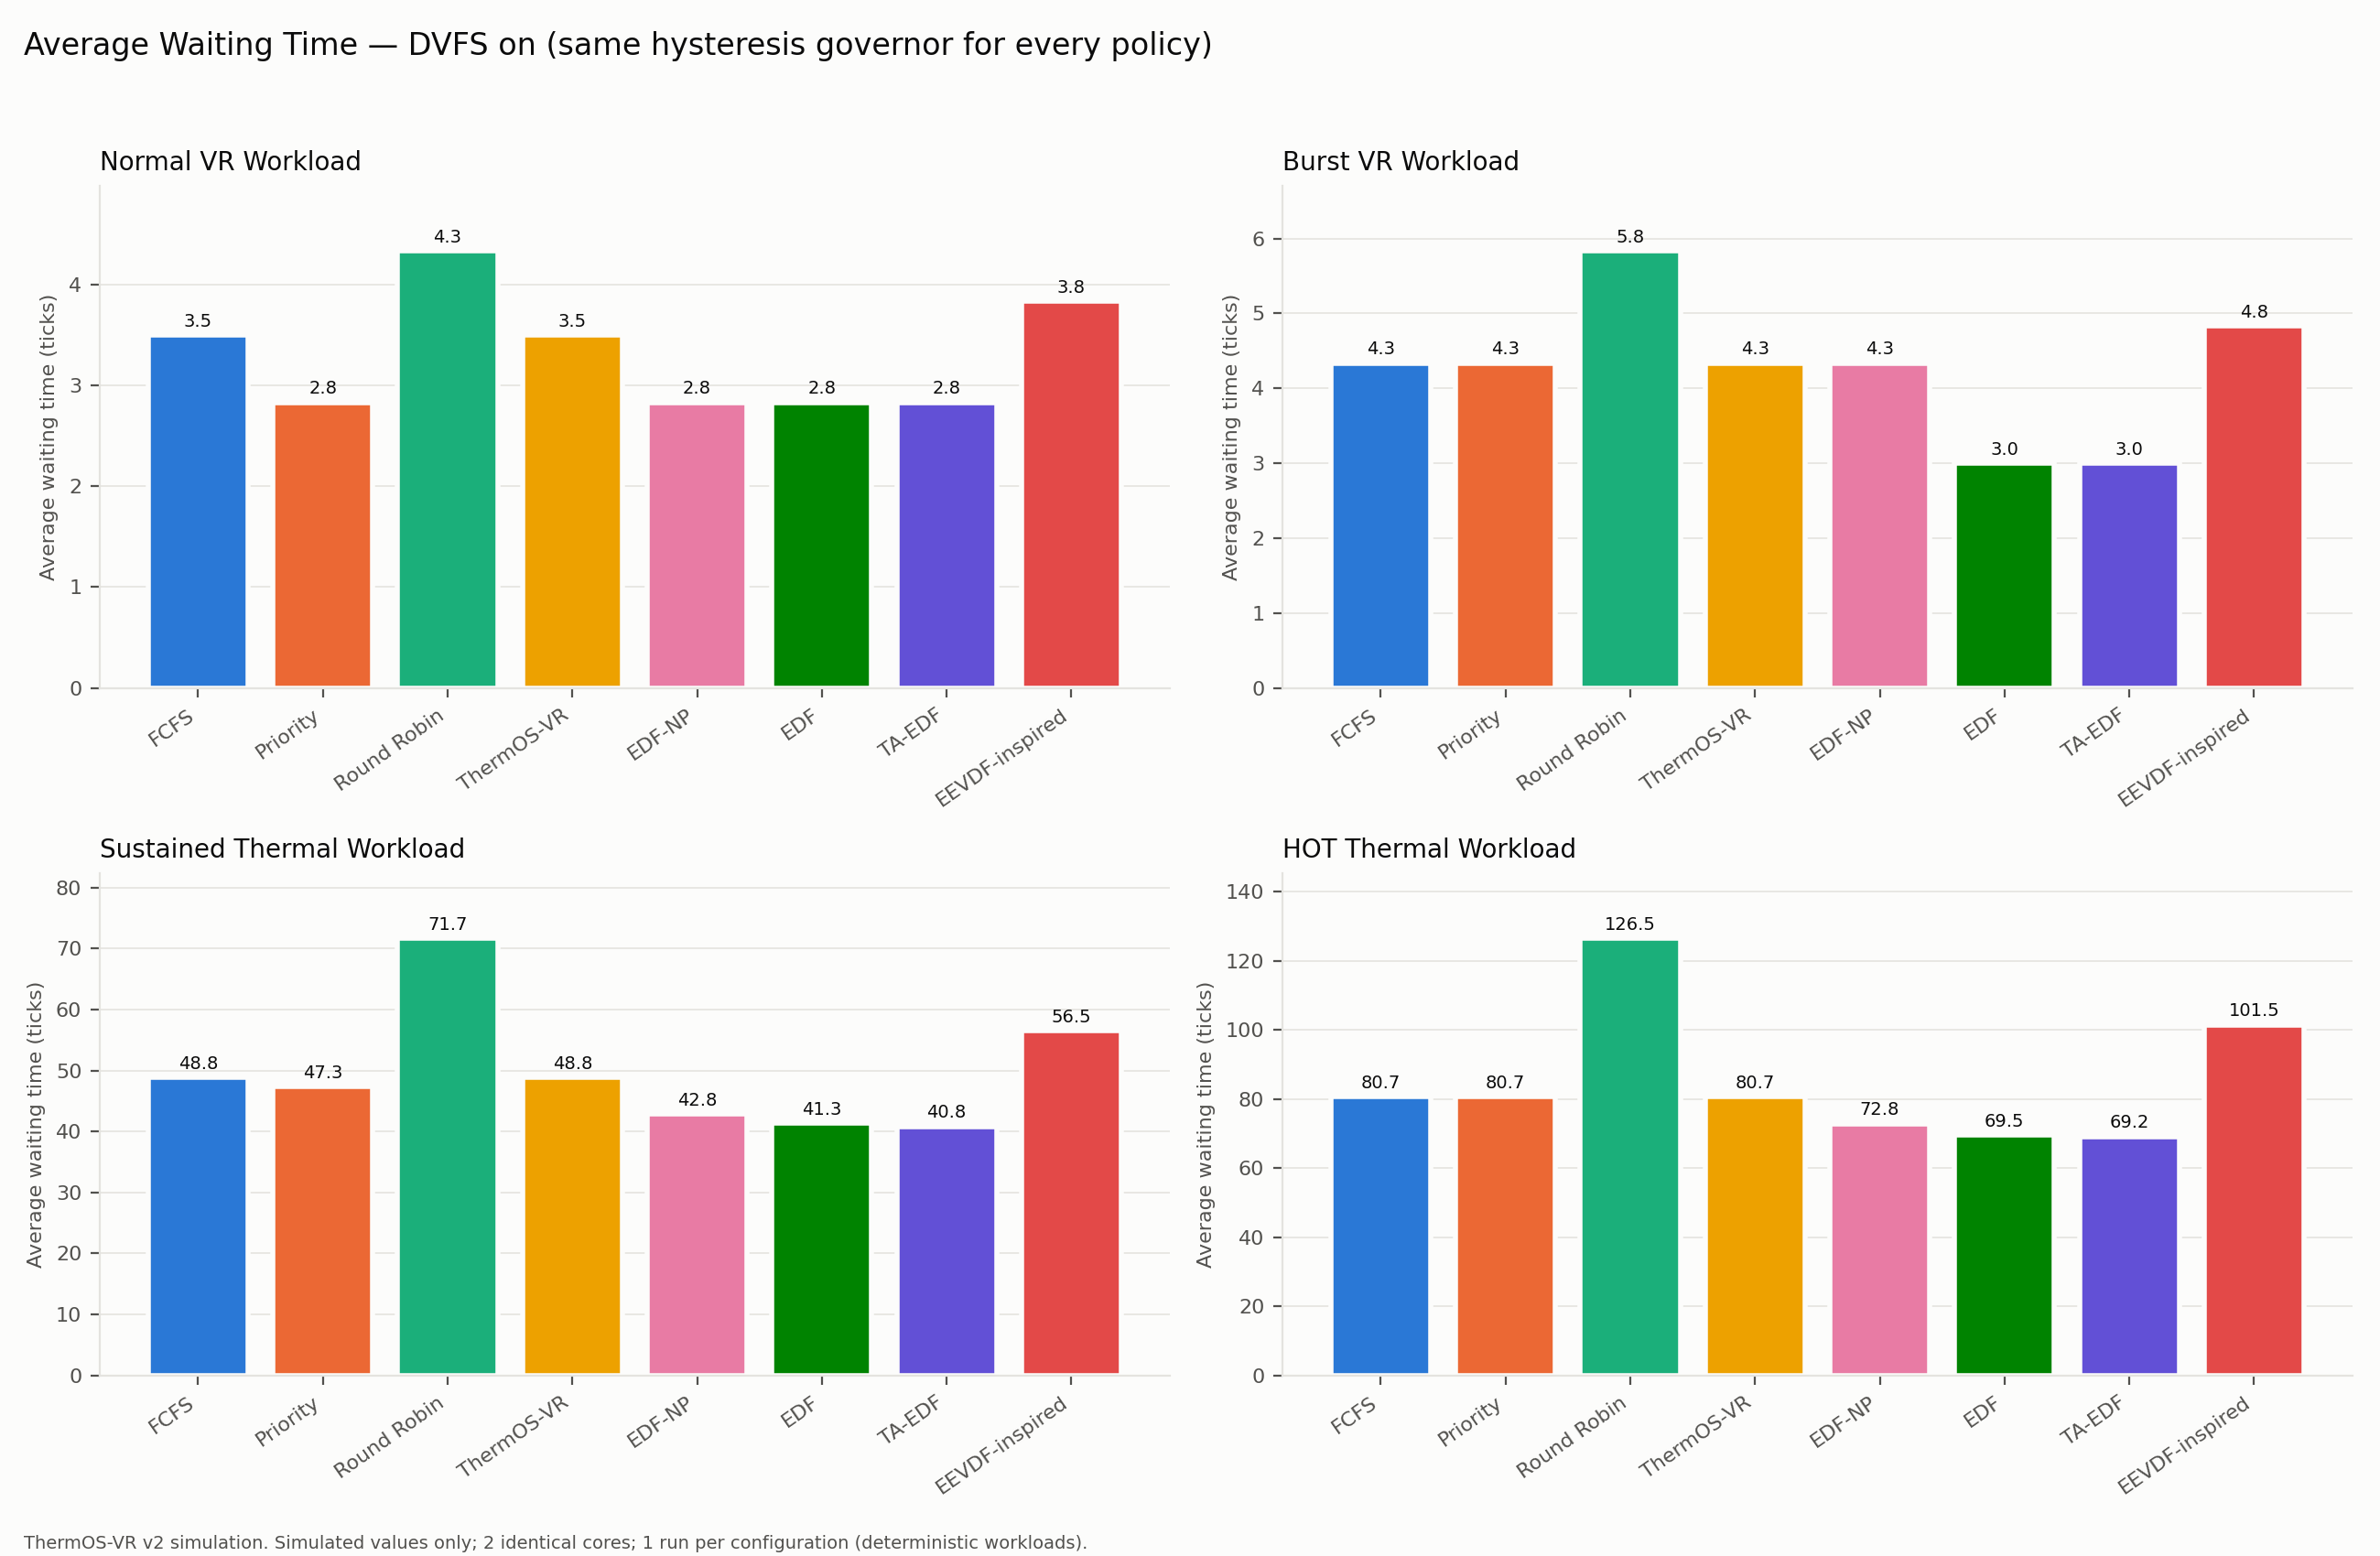
\includegraphics[width=\textwidth]{figures/hysteresis_waiting_time.png}
\caption{Average waiting time (ticks), DVFS enabled, one deterministic run per policy and workload. FCFS and ThermOS-VR are identical by construction; ties occur in Normal VR.}
\label{fig:wait}
\end{figure*}

Preemption mattered: EDF-NP improved on FCFS, Priority and ThermOS-VR only in Sustained and HOT Thermal, and tied them in Burst VR (4.33 ticks). Round Robin had the highest waiting time and the highest total tardiness in every configuration (for example, a tardiness of 697 ticks in HOT Thermal with DVFS enabled, against 368 for EDF), and the EEVDF-inspired policy had the second-highest waiting time everywhere. Both missed all six deadlines in Sustained and HOT Thermal, whereas every other policy missed four. Fig.~\ref{fig:tard} shows the corresponding tardiness values. With DVFS disabled the same pattern held (Table~\ref{tab:thermoff}): the EDF variants again had the lowest values and Round Robin and the EEVDF-inspired policy the highest waiting times. EDF and TA-EDF tied in Sustained Thermal (waiting 39.17 ticks, tardiness 182) and on tardiness in HOT Thermal (305), and EDF had the lower waiting time in HOT Thermal (64.17 versus 64.33 ticks).

\begin{figure*}[!t]
\centering
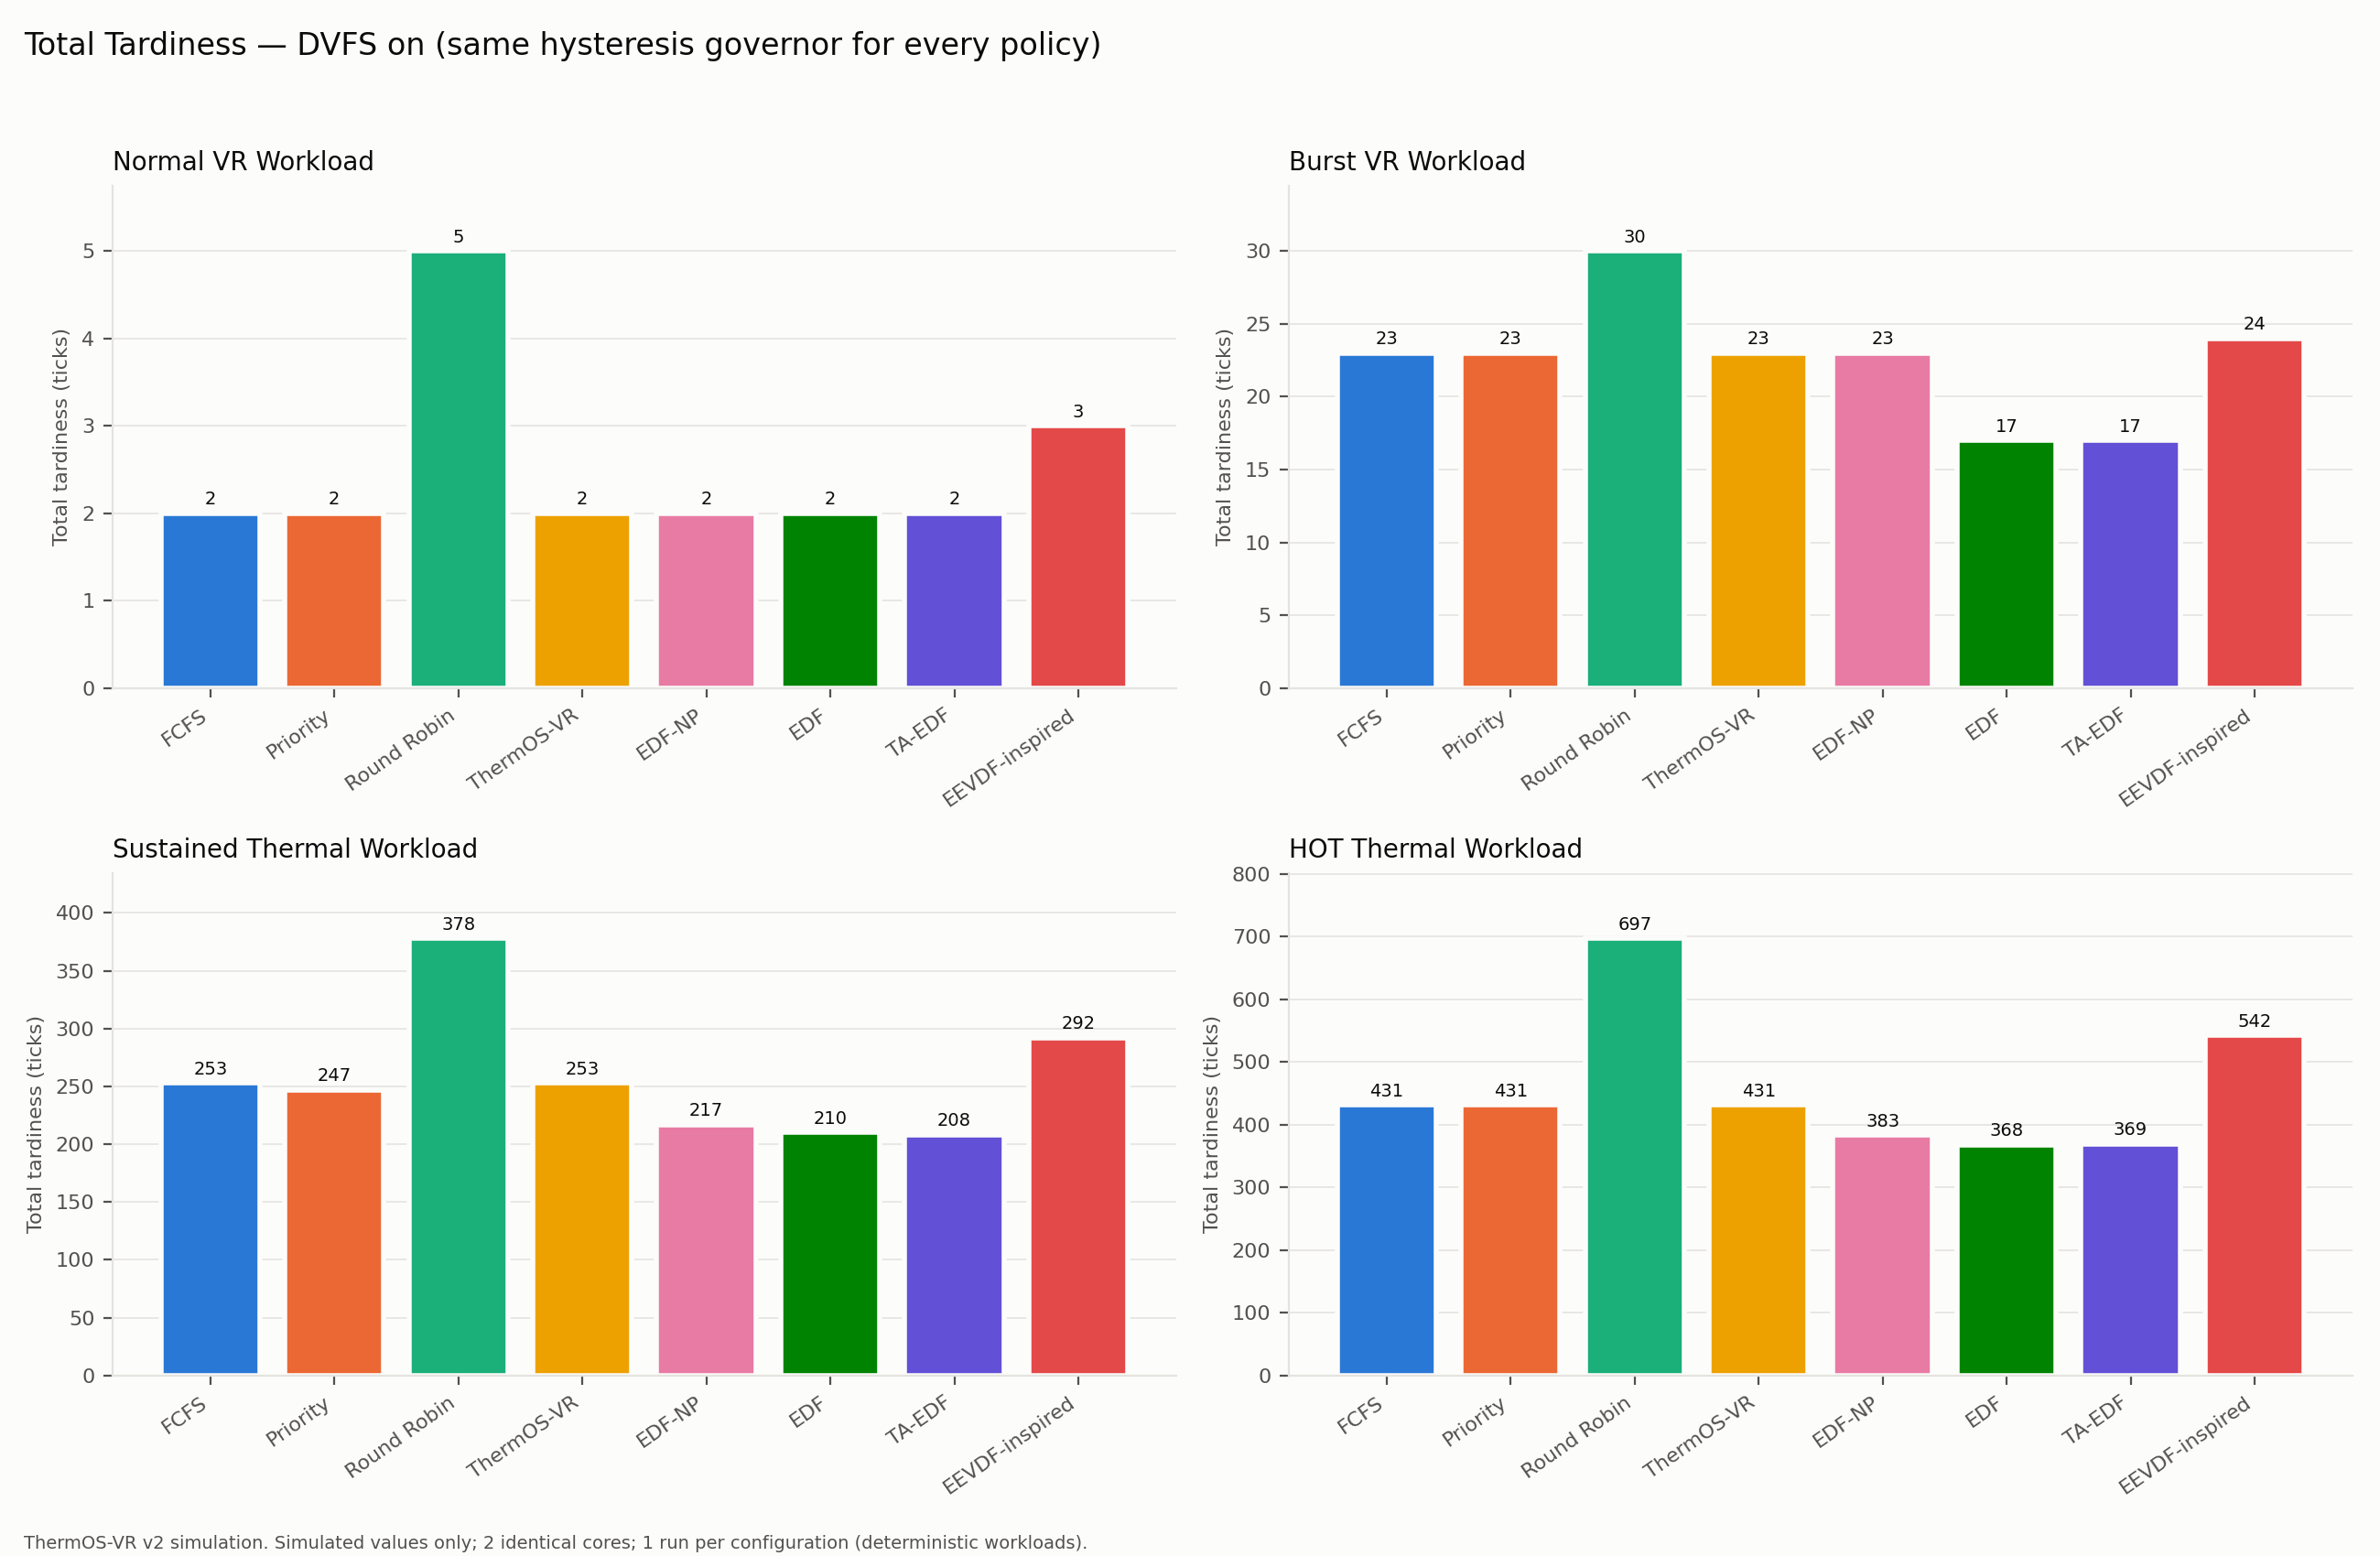
\includegraphics[width=\textwidth]{figures/hysteresis_total_tardiness.png}
\caption{Total tardiness (ticks), DVFS enabled. Tasks are not dropped after missing a deadline; Burst, Sustained and HOT are partly infeasible on two cores.}
\label{fig:tard}
\end{figure*}

\subsection{Simulated Thermal Behaviour}\label{sec:res-thermal}
With DVFS enabled (Table~\ref{tab:thermon}), no policy reached the HOT state in any workload. This is a consequence of the modelled governor and parameters (a loaded core settles near 63.7 \textdegree{}C at 2.2 GHz) and says nothing about the thermal safety of real hardware. Core-ticks at or above 60 \textdegree{}C separated the policies more clearly (Fig.~\ref{fig:ge60}): in Sustained Thermal they ranged from 5 for Round Robin and 28 for TA-EDF to 108 for EDF, and in HOT Thermal from 49 for Round Robin and 257 for TA-EDF to 286 for EDF. Round Robin achieves its low values by interleaving light and heavy tasks, at the cost of the worst responsiveness reported above.

\begin{table*}[!t]
\centering
\scriptsize
\caption{Simulated thermal outcomes with DVFS enabled (model \textdegree{}C, core-ticks). Peak: N, B, S, H workloads; other columns: Sustained and HOT only, because Normal and Burst never reach 60 \textdegree{}C. No run reached the HOT state.}
\label{tab:thermon}
\setlength{\tabcolsep}{3pt}
\begin{tabular}{lrrrrrrrrrrrr}
\toprule
Policy & \multicolumn{4}{c}{Peak \textdegree{}C} & \multicolumn{2}{c}{Core-ticks $\geq$ 60 \textdegree{}C} & \multicolumn{2}{c}{Throttled busy core-ticks} & \multicolumn{2}{c}{Migrations} & \multicolumn{2}{c}{Makespan} \\
\cmidrule(lr){2-5} \cmidrule(lr){6-7} \cmidrule(lr){8-9} \cmidrule(lr){10-11} \cmidrule(lr){12-13}
 & N & B & S & H & Sus & HOT & Sus & HOT & Sus & HOT & Sus & HOT \\
\midrule
FCFS & 49.10 & 57.24 & 61.28 & 62.49 & 107 & 281 & 142 & 304 & 0 & 0 & 135 & 226 \\
Priority & 50.59 & 57.24 & 61.28 & 62.49 & 102 & 281 & 137 & 304 & 0 & 0 & 134 & 226 \\
RR & 48.20 & 57.65 & 60.25 & 61.02 & 5 & 49 & 123 & 338 & 35 & 52 & 131 & 224 \\
ThermOS-VR & 49.10 & 57.24 & 61.28 & 62.49 & 107 & 281 & 142 & 304 & 0 & 0 & 135 & 226 \\
EDF-NP & 50.59 & 57.24 & 61.28 & 63.11 & 90 & 269 & 116 & 291 & 0 & 0 & 131 & 224 \\
EDF & 50.59 & 57.58 & 61.28 & 63.33 & 108 & 286 & 134 & 294 & 0 & 0 & 133 & 224 \\
TA-EDF & 48.10 & 57.50 & 60.24 & 62.34 & 28 & 257 & 123 & 321 & 77 & 193 & 133 & 223 \\
EEVDF-insp. & 50.41 & 58.16 & 61.40 & 62.88 & 77 & 282 & 146 & 294 & 33 & 132 & 142 & 244 \\
\bottomrule
\end{tabular}
\end{table*}

\begin{figure*}[!t]
\centering
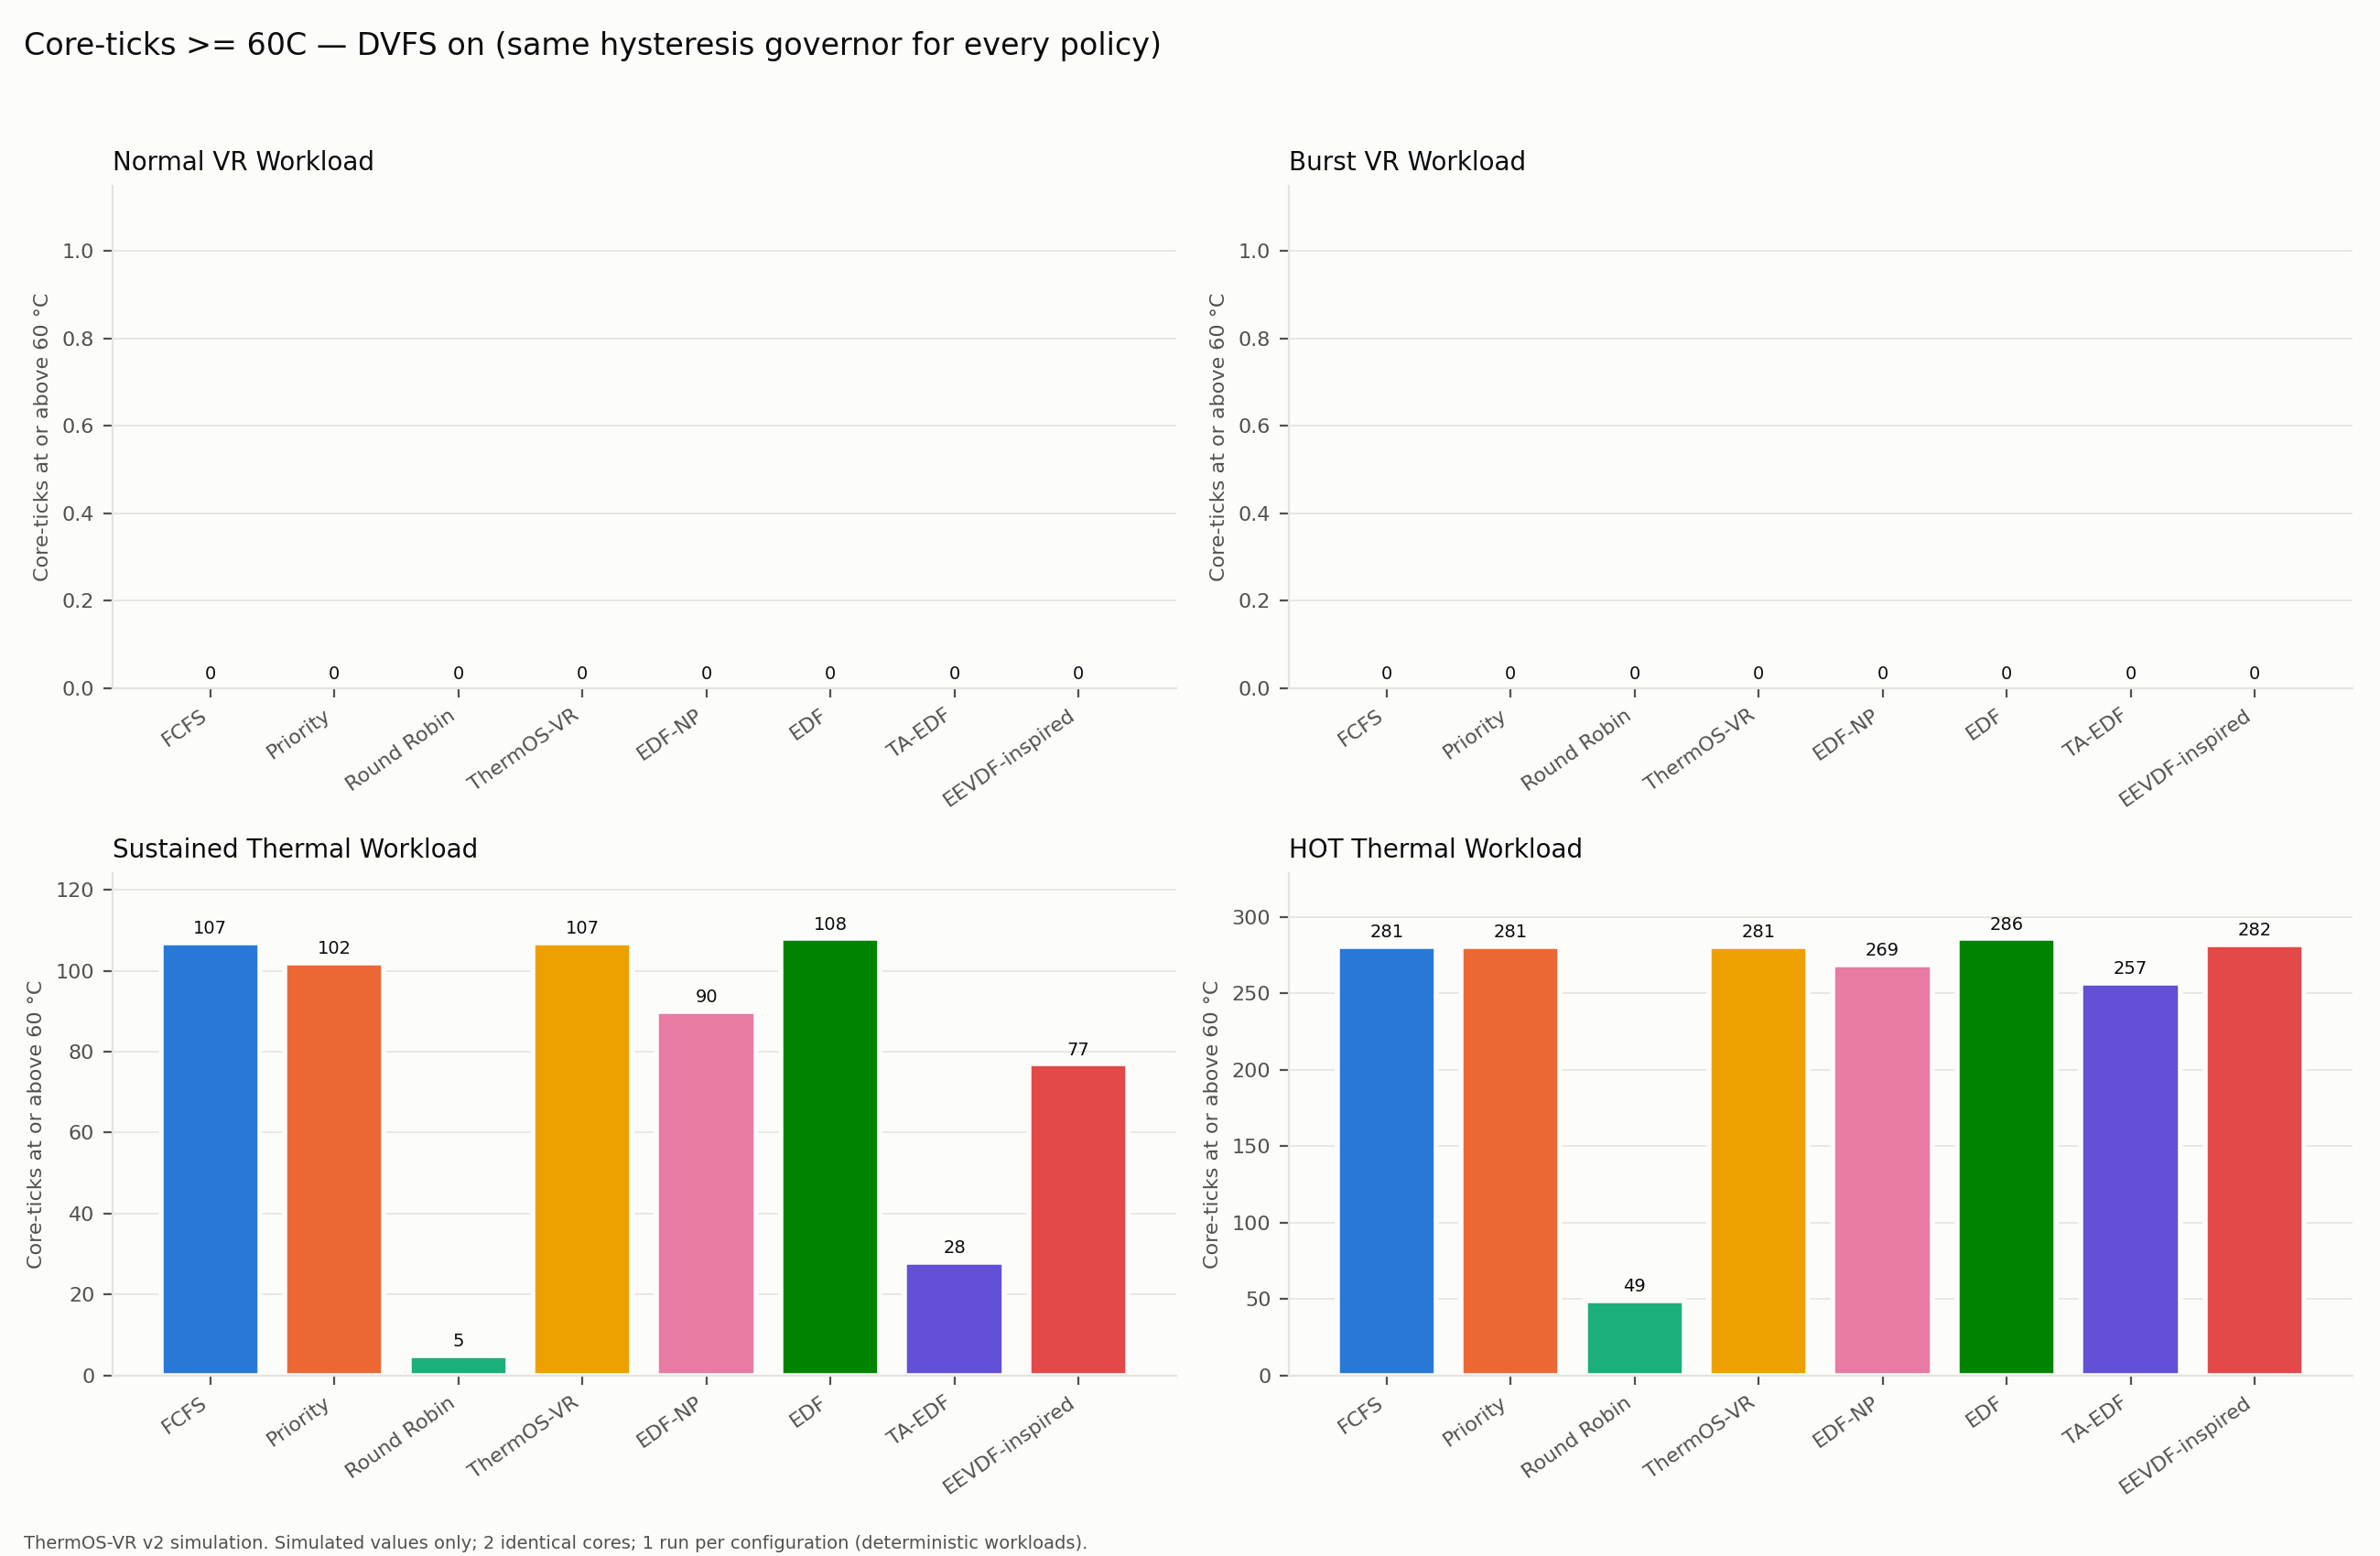
\includegraphics[width=\textwidth]{figures/hysteresis_core_ticks_above_60c.png}
\caption{Core-ticks at or above the 60 \textdegree{}C model threshold, DVFS enabled. Values are simulated by the simplified thermal model; Normal and Burst never reach 60 \textdegree{}C.}
\label{fig:ge60}
\end{figure*}

At zero overhead, TA-EDF's simulated peak temperature was below EDF's in all eight configurations (Fig.~\ref{fig:peak}), by between 0.08 \textdegree{}C (Burst VR) and 2.49 \textdegree{}C (Normal VR). The reduction came with more throttling in one case: in HOT Thermal with DVFS enabled, TA-EDF spent 321 busy core-ticks below 2.5 GHz against 294 for EDF, because it kept both cores near the 60 \textdegree{}C threshold.

\begin{figure*}[!t]
\centering
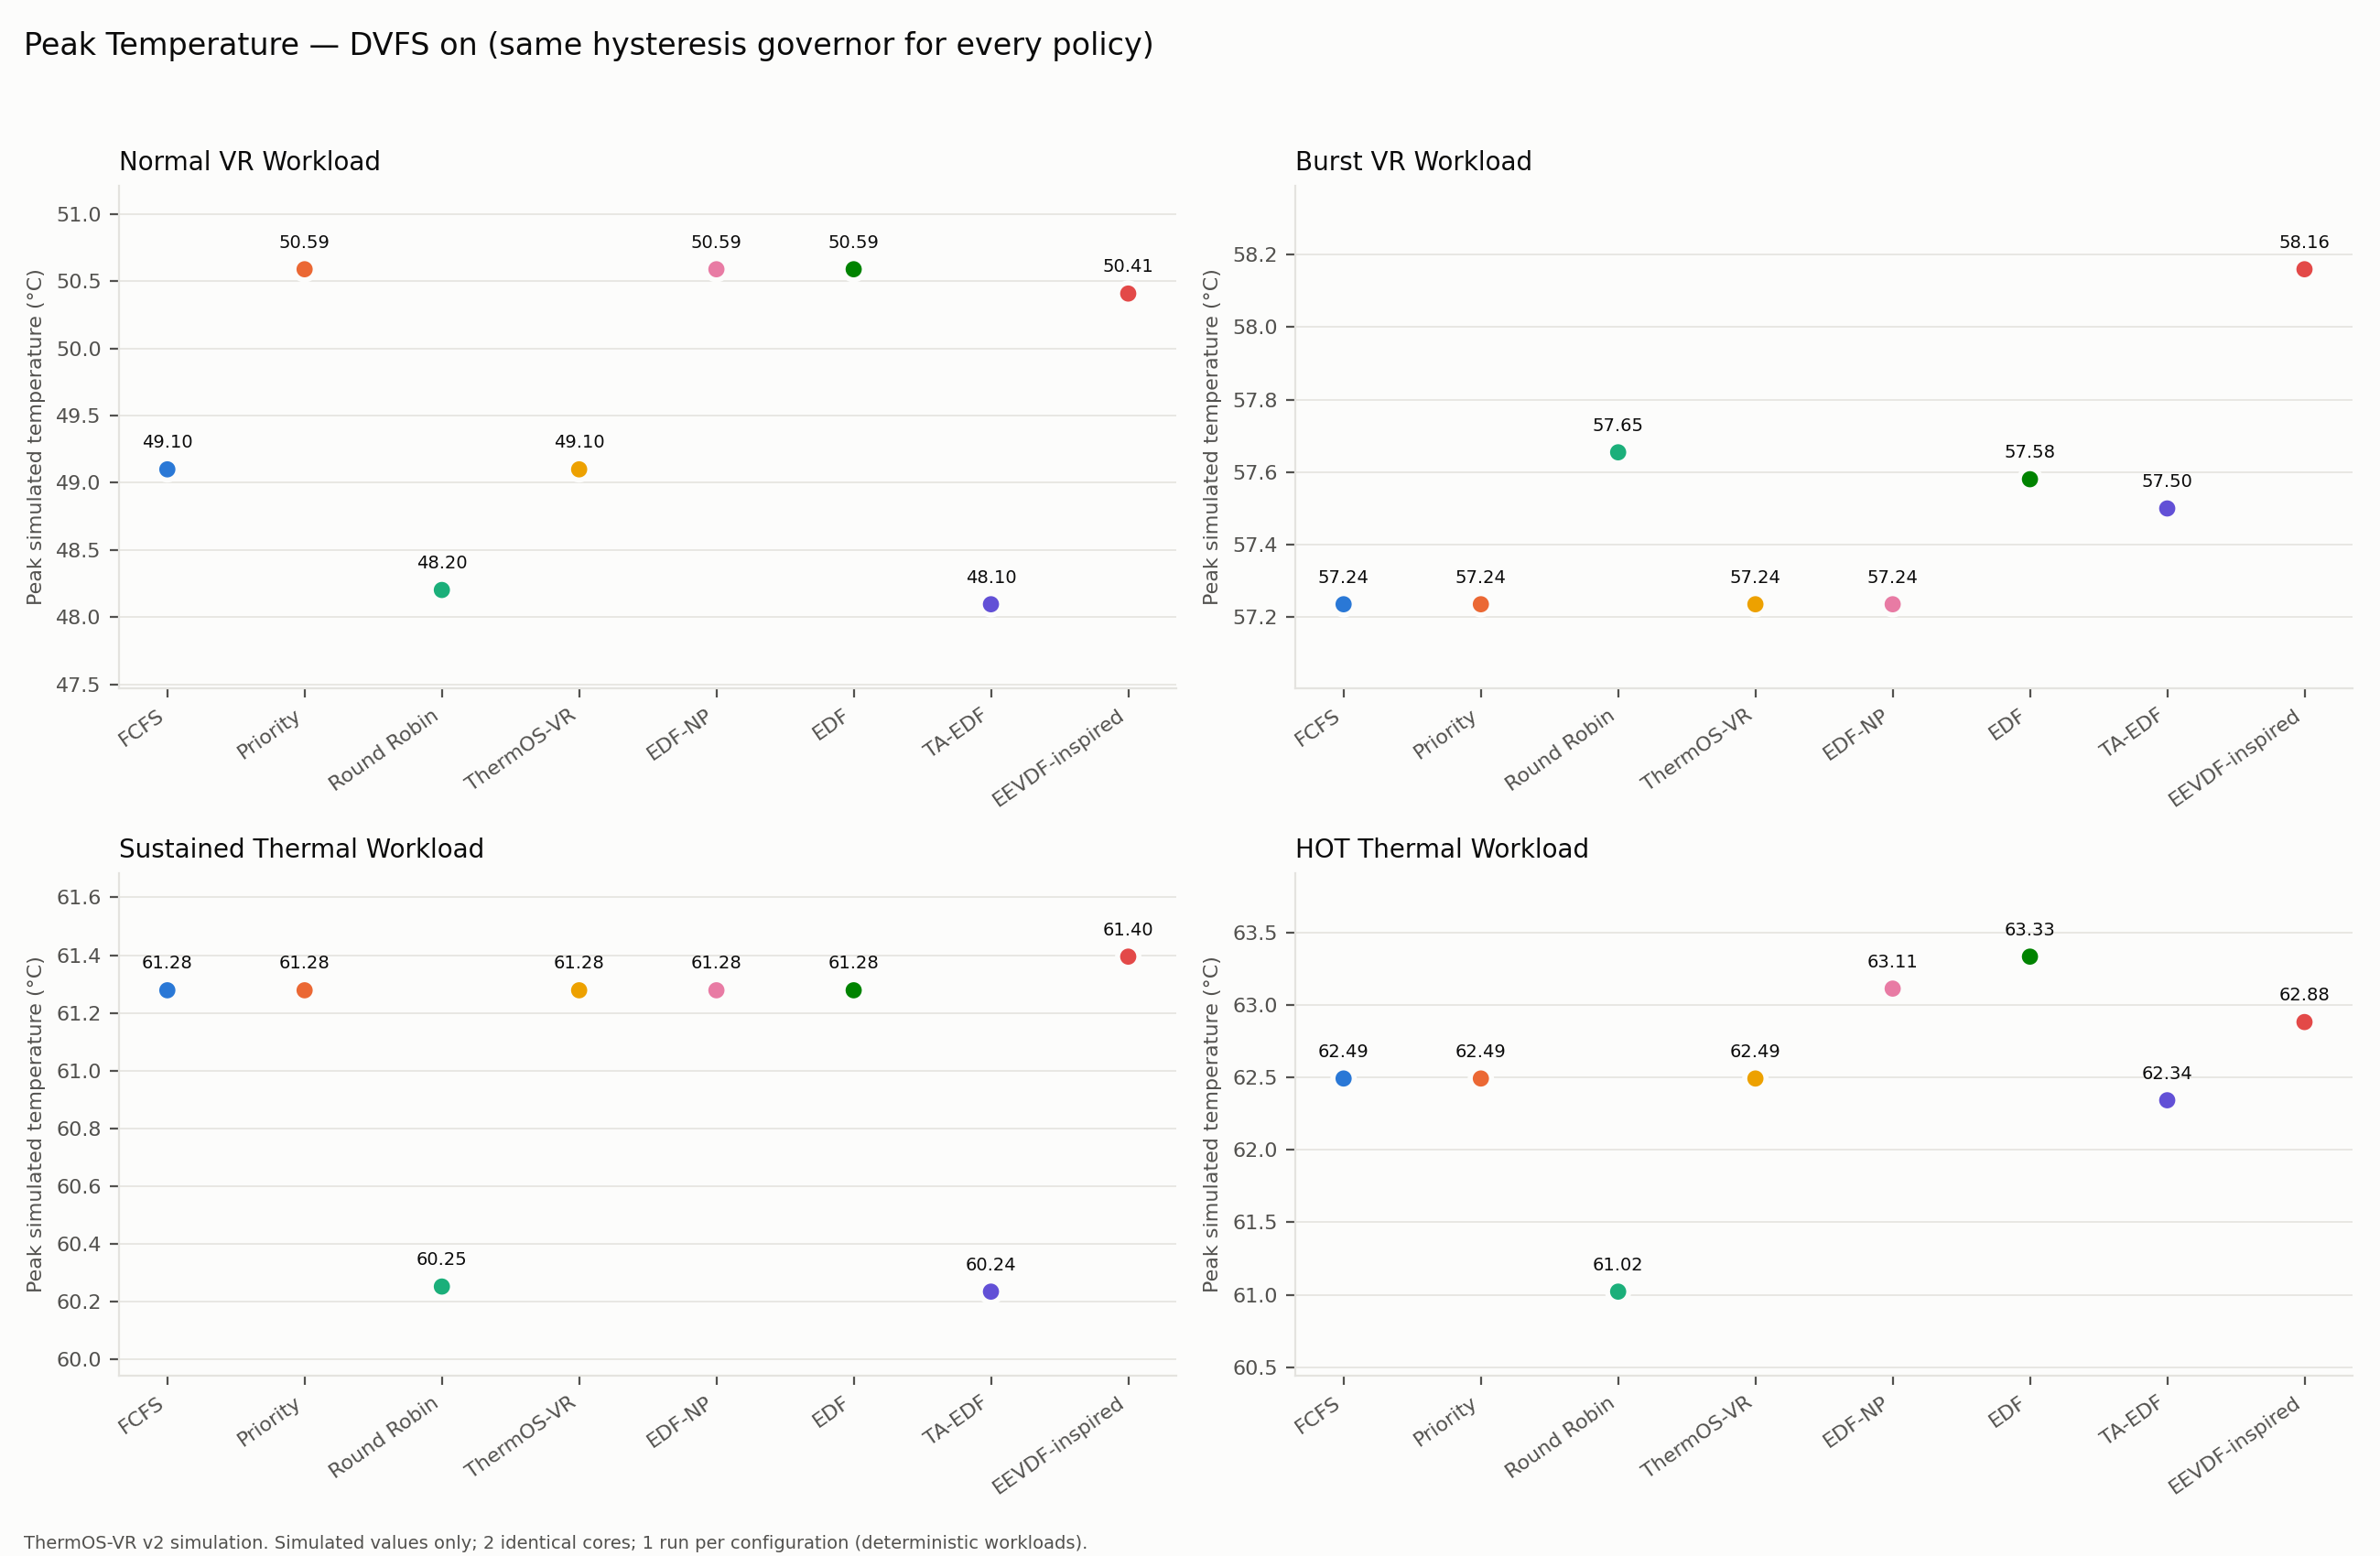
\includegraphics[width=\textwidth]{figures/hysteresis_peak_temperature.png}
\caption{Peak simulated temperature (model \textdegree{}C), DVFS enabled. Dot plot because the axis does not start at zero; differences are small and come from single deterministic runs.}
\label{fig:peak}
\end{figure*}

With DVFS disabled (Table~\ref{tab:thermoff}), only the HOT workload entered the HOT state. HOT core-ticks were 18 for Round Robin, 26 for TA-EDF, 35 for EDF-NP, 64 for FCFS, Priority and ThermOS-VR, 65 for EDF and 104 for the EEVDF-inspired policy. Core-ticks at or above 60 \textdegree{}C did not follow the same ordering: TA-EDF had more than EDF in Sustained (154 versus 137) and HOT Thermal (304 versus 299). Total model heat was identical for every policy within each workload (18.20, 58.00, 205.00 and 359.25 model units for Normal, Burst, Sustained and HOT).

\begin{table*}[!t]
\centering
\scriptsize
\caption{DVFS disabled (fixed 2.5 GHz), Sustained (Sus) and HOT workloads. Total model heat is identical for all policies in each workload.}
\label{tab:thermoff}
\setlength{\tabcolsep}{3pt}
\begin{tabular}{lrrrrrrrrr}
\toprule
Policy & \multicolumn{2}{c}{Peak \textdegree{}C} & HOT c.-t. & \multicolumn{2}{c}{$\geq$ 60 \textdegree{}C} & \multicolumn{2}{c}{Waiting} & \multicolumn{2}{c}{Tardiness} \\
\cmidrule(lr){2-3} \cmidrule(lr){5-6} \cmidrule(lr){7-8} \cmidrule(lr){9-10}
 & Sus & HOT & HOT & Sus & HOT & Sus & HOT & Sus & HOT \\
\midrule
FCFS & 67.61 & 71.74 & 64 & 170 & 341 & 45.00 & 72.50 & 215 & 355 \\
Priority & 67.92 & 71.74 & 64 & 165 & 341 & 44.17 & 72.50 & 212 & 355 \\
RR & 67.11 & 71.26 & 18 & 109 & 310 & 67.67 & 114.00 & 338 & 579 \\
ThermOS-VR & 67.61 & 71.74 & 64 & 170 & 341 & 45.00 & 72.50 & 215 & 355 \\
EDF-NP & 67.11 & 72.49 & 35 & 121 & 332 & 40.83 & 66.67 & 192 & 320 \\
EDF & 68.48 & 73.64 & 65 & 137 & 299 & 39.17 & 64.17 & 182 & 305 \\
TA-EDF & 66.66 & 71.67 & 26 & 154 & 304 & 39.17 & 64.33 & 182 & 305 \\
EEVDF-insp. & 67.25 & 72.35 & 104 & 157 & 335 & 52.50 & 91.50 & 247 & 444 \\
\bottomrule
\end{tabular}
\end{table*}

\subsection{What TA-EDF Actually Did}\label{sec:res-mech}
TA-EDF migrated tasks frequently: 8, 41, 77 and 193 times in Normal, Burst, Sustained and HOT with DVFS enabled (8, 41, 64 and 114 with DVFS disabled), whereas EDF never migrated a task. Its hold-back rule, by contrast, never left a core idle in any of the 64 runs. In each DVFS setting, a core at or above 59 \textdegree{}C coexisted with a task of sufficient slack in 31 ticks (3 in Sustained and 28 in HOT). In 31 cases that task was offered the other, cooler core and ran there; in 9 cases earlier-deadline tasks had already filled both cores; and once (HOT, tick 32) the task was skipped but the next EDF candidate took the core immediately. In these workloads, by the time cores are warm most tasks have little or negative slack, so the condition for idling a core never arises. TA-EDF's observed behaviour is therefore effectively preemptive EDF with migration-based coolest-core placement; the idle-insertion rule remains untested.

The per-core temperature traces of the HOT workload (Fig.~\ref{fig:trace}) show what this placement does. We summarise them by the mean absolute temperature difference between the two cores over the run, computed from the per-tick trace. With DVFS enabled it was 3.22 \textdegree{}C for EDF and 1.43 \textdegree{}C for TA-EDF, so coolest-core placement reduced the imbalance that EDF's sticky placement creates by more than half; with DVFS disabled the values were 5.58 and 3.01 \textdegree{}C. FCFS, however, kept the cores even closer (0.72 \textdegree{}C with DVFS enabled), plausibly because its non-preemptive order runs similar heavy tasks side by side. Thermal balance alone is therefore not a distinguishing property of TA-EDF.

\begin{figure*}[!t]
\centering
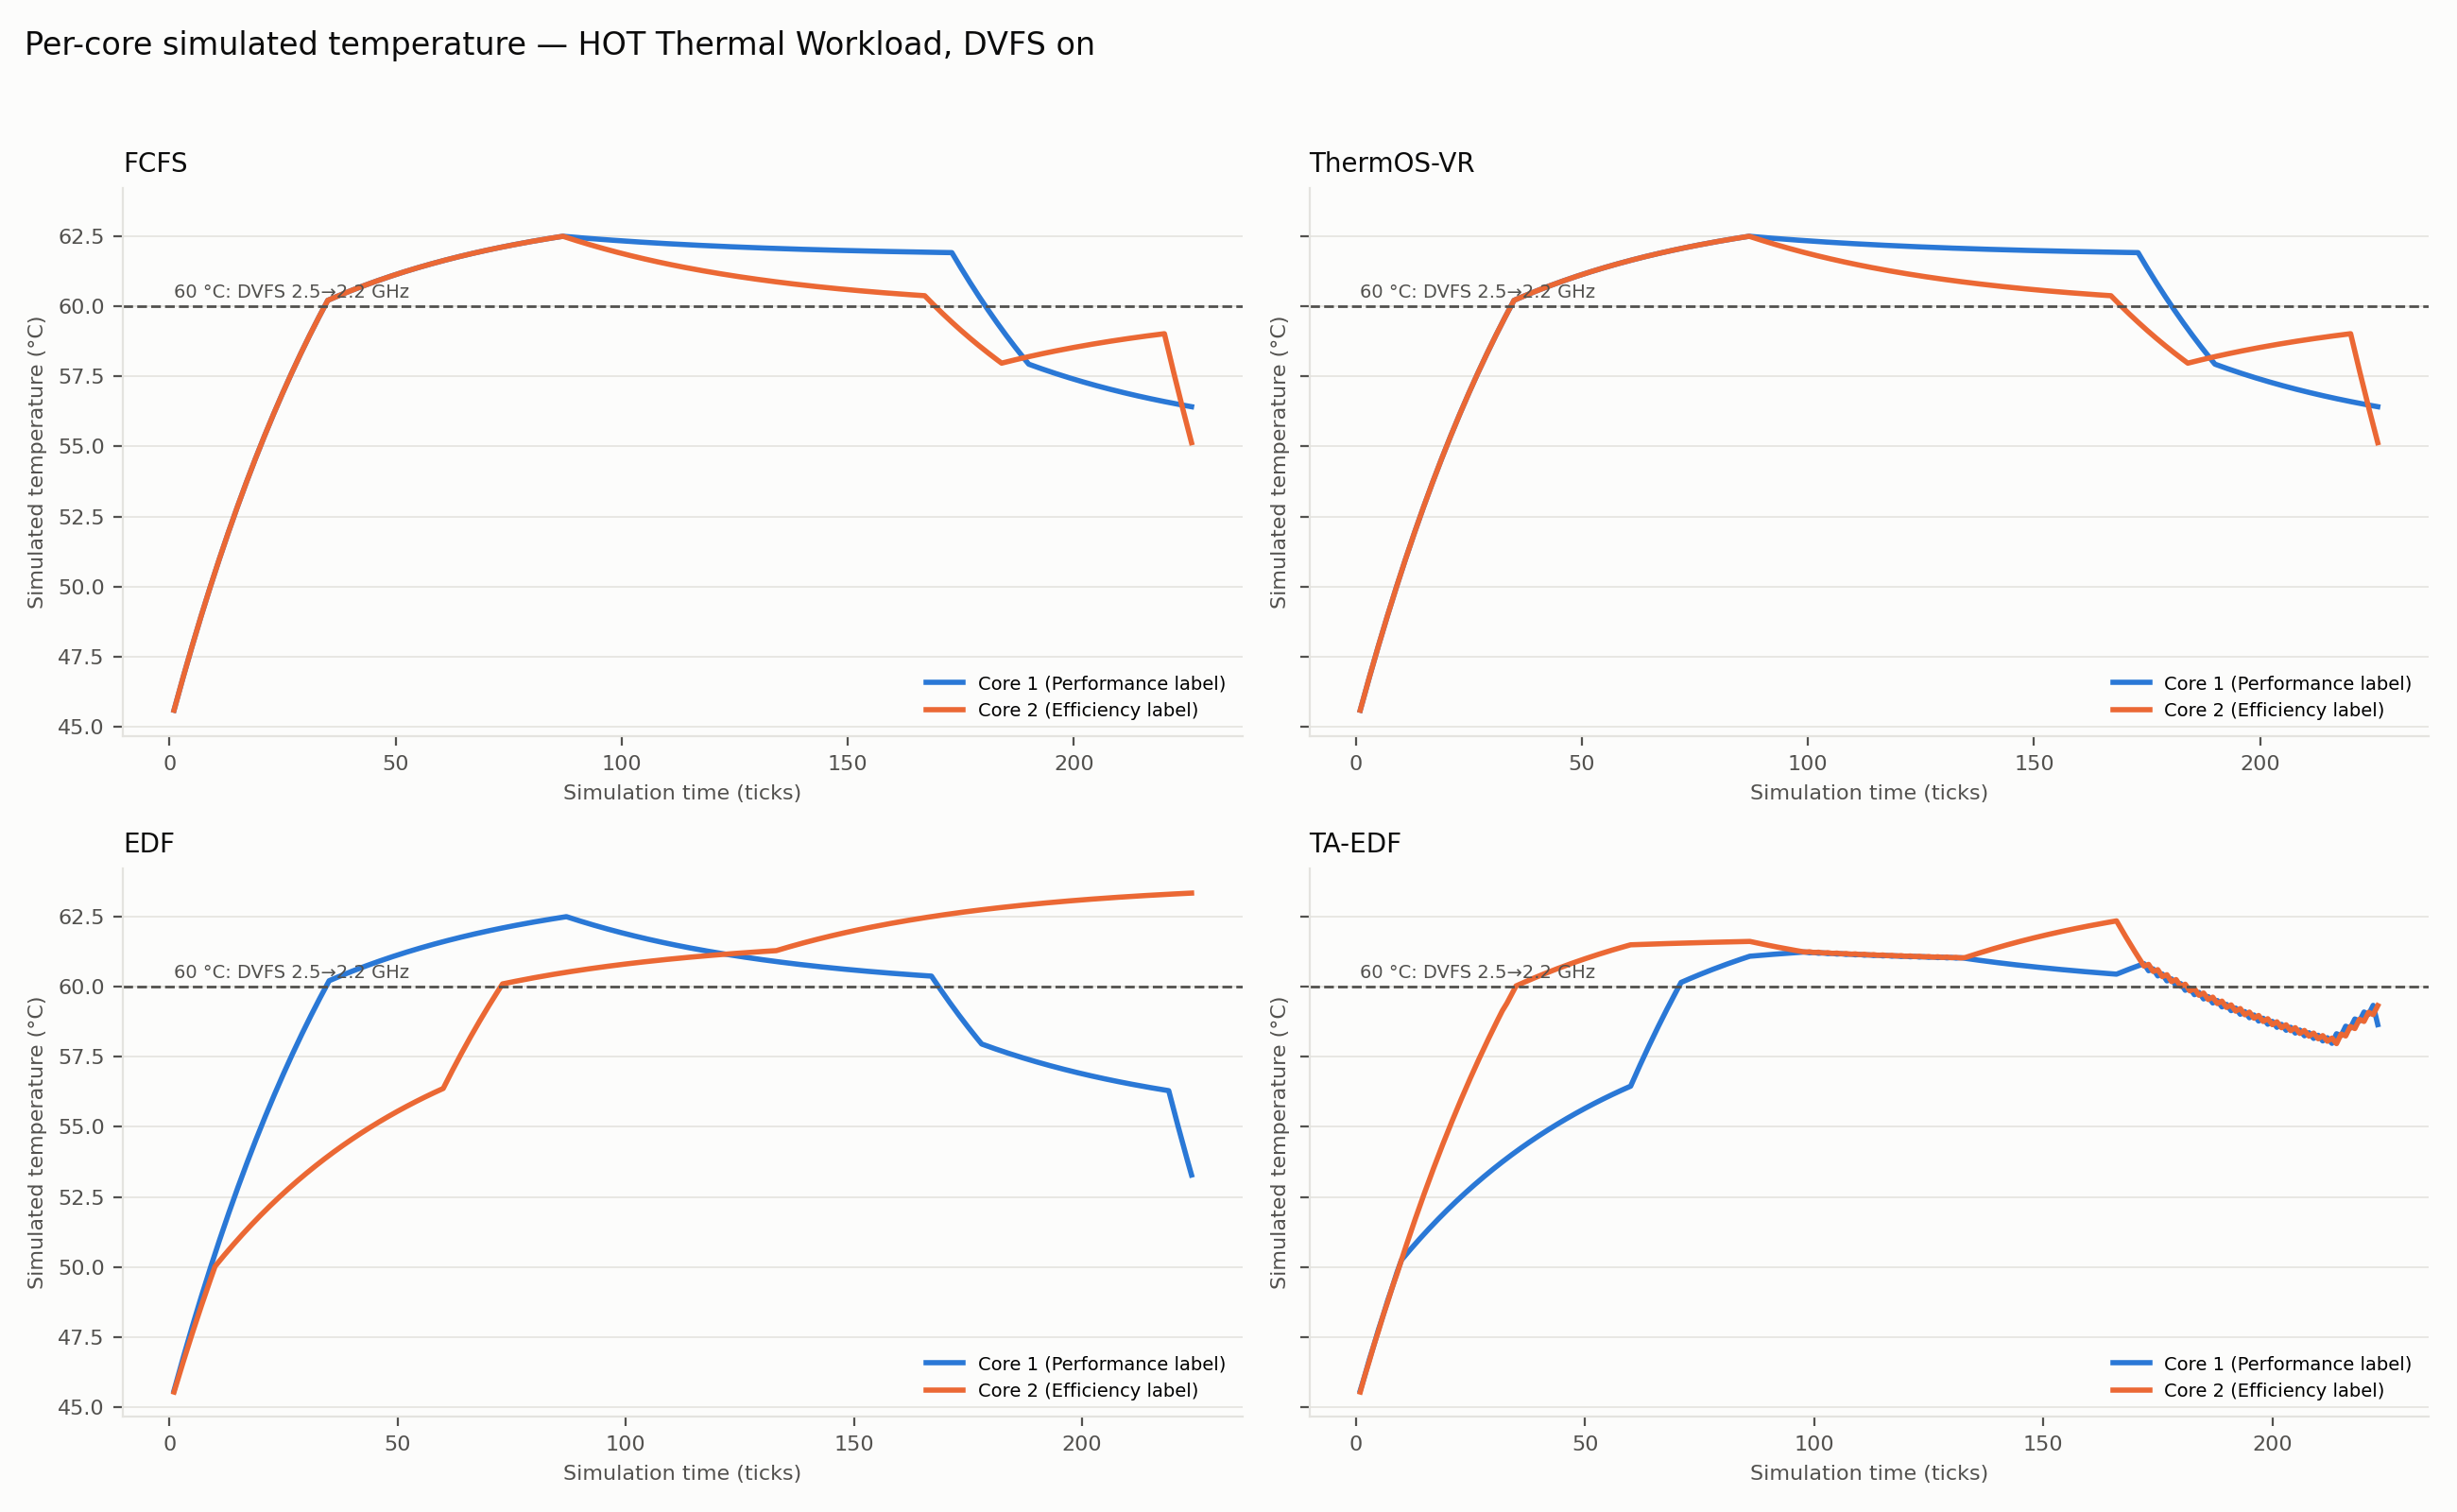
\includegraphics[width=\textwidth]{figures/hysteresis_hot_temperature_trace.png}
\caption{Per-core simulated temperature over time (model \textdegree{}C), HOT workload, DVFS enabled, for FCFS, ThermOS-VR, EDF and TA-EDF. The FCFS and ThermOS-VR panels are identical by construction; the dashed line is the governor's first threshold.}
\label{fig:trace}
\end{figure*}

\subsection{Sensitivity to Migration and Context-Switch Costs}\label{sec:res-sens}
Because EDF never migrated, its results were almost unaffected by the overhead costs: its total tardiness changed by at most 2 ticks across the whole cost grid. TA-EDF behaved differently (Table~\ref{tab:sens}, Fig.~\ref{fig:sens}). With zero migration cost, TA-EDF and EDF differed by at most 5 ticks of tardiness whatever the context-switch cost (range $-$4 to +5). For every migration cost of at least 0.1 work units, however, TA-EDF had higher total tardiness and a longer makespan than EDF in all 96 matched configurations, with differences of +1 to +365 ticks in tardiness and +2 to +121 ticks in makespan. At migration costs of 0.25 and above it also missed three to four more deadlines than EDF in Burst VR, and at 0.5 with DVFS enabled one more in HOT Thermal.

\begin{table*}[!t]
\centering
\scriptsize
\caption{TA-EDF minus EDF at each migration cost (simulated work units; context-switch cost 0), matched on workload (N, B, S, H) and DVFS setting. Positive $\Delta$ tardiness or makespan means TA-EDF is worse.}
\label{tab:sens}
\setlength{\tabcolsep}{3pt}
\begin{tabular}{lrrrrrrrrrrrr}
\toprule
DVFS, cost & \multicolumn{4}{c}{$\Delta$ tardiness (ticks)} & \multicolumn{4}{c}{$\Delta$ makespan (ticks)} & \multicolumn{4}{c}{$\Delta$ peak (\textdegree{}C)} \\
\cmidrule(lr){2-5} \cmidrule(lr){6-9} \cmidrule(lr){10-13}
 & N & B & S & H & N & B & S & H & N & B & S & H \\
\midrule
on, 0 & 0 & 0 & -2 & +1 & 0 & 0 & 0 & -1 & -2.49 & -0.08 & -1.04 & -0.99 \\
on, 0.1 & +1 & +8 & +13 & +37 & +2 & +4 & +6 & +12 & -2.09 & +1.05 & -1.08 & -1.06 \\
on, 0.25 & +2 & +24 & +39 & +113 & +2 & +9 & +16 & +39 & -2.09 & +2.22 & -1.09 & -1.10 \\
on, 0.5 & +4 & +71 & +159 & +365 & +4 & +21 & +61 & +121 & -2.02 & +2.97 & -1.18 & -1.11 \\
\midrule
off, 0 & 0 & 0 & 0 & 0 & 0 & 0 & 0 & -1 & -2.49 & -0.08 & -1.82 & -1.97 \\
off, 0.1 & +1 & +8 & +13 & +19 & +2 & +4 & +5 & +8 & -2.09 & +1.05 & -1.64 & -2.08 \\
off, 0.25 & +2 & +24 & +28 & +46 & +2 & +9 & +12 & +20 & -2.09 & +2.22 & -1.58 & -1.98 \\
off, 0.5 & +4 & +67 & +67 & +118 & +4 & +19 & +32 & +56 & -2.02 & +3.93 & -1.51 & -2.00 \\
\bottomrule
\end{tabular}
\end{table*}

\begin{figure}[!t]
\centering
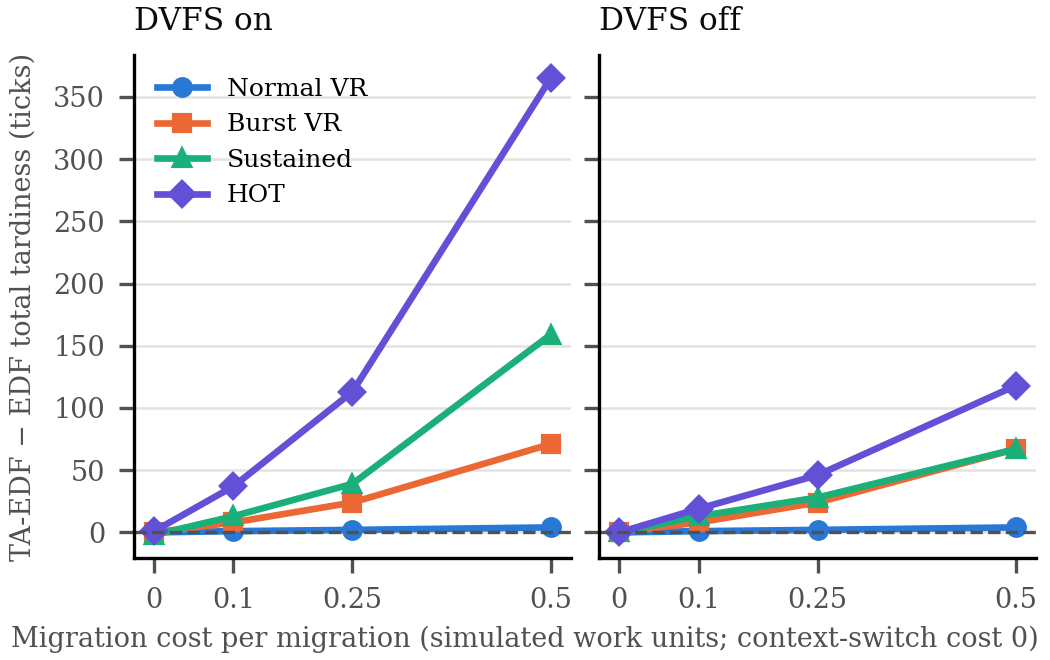
\includegraphics[width=\columnwidth]{figures/fig_sensitivity_tardiness.png}
\caption{TA-EDF minus EDF total tardiness versus migration cost (context-switch cost 0), matched on workload and DVFS setting. Positive values mean TA-EDF is later. Costs are hypothetical simulated work units, not measured latencies.}
\label{fig:sens}
\end{figure}

The thermal side of the trade-off persisted in three of the four workloads: in Normal, Sustained and HOT, TA-EDF's simulated peak stayed 0.99--2.49 \textdegree{}C below EDF's at every cost. In Burst VR, once migrations cost anything, TA-EDF's peak was 0.70--3.93 \textdegree{}C \emph{above} EDF's; we did not investigate the mechanism behind this reversal. The zero-overhead rows of this experiment reproduced the main benchmark exactly (64 runs $\times$ 16 metrics).

\subsection{EEVDF-Inspired Policy on One and Two Cores}\label{sec:res-eevdf}
On a single core the EEVDF-inspired policy never dispatched an ineligible task, and the largest lag observed was between 0.73 and 0.94 slices, consistent with the one-quantum bound of the original algorithm~\cite{stoica1995}. On two cores it dispatched ineligible tasks in 4, 15, 27 and 56 ticks of the Normal, Burst, Sustained and HOT workloads (DVFS enabled), and the largest lag reached 2.26, 3.55, 7.67 and 22.59 slices respectively. This behaviour follows from combining a global queue, a work-conserving rule and weight ratios of up to 87:1, under which a heavy task's fair share can exceed one core; it mirrors the infeasible-weight problem described for symmetric multiprocessors~\cite{chandra2000}. The two-core results of this policy therefore carry no fairness guarantee.

\section{Discussion}\label{sec:discussion}
\emph{Why ThermOS-VR equals FCFS.} The score in \eqref{eq:score} can only choose between identical idle cores, and its deadline term is constant across them. With FCFS ordering and no preemption, the start and finish time of every task is fixed before any core is chosen. Because the cores are identical, swapping two tasks between them changes only which core carries which heat trace, and every aggregate metric is symmetric in the two cores. A thermal score can matter only when cores differ in temperature in a way that changes future speed, which in this model requires DVFS, and even then the FCFS order leaves little room for it to act.

\emph{Why DVFS dominates the thermal results.} The thermal update is linear and the cores are identical, so with a fixed frequency the total heat a workload produces is fixed by its work, and the average temperature can change only through the timing of that work. Placement can redistribute heat between cores, which changes the peak and the threshold-based counts, but it cannot reduce the total. Lowering the frequency reduces the heat per tick quadratically while reducing progress linearly, which is why the governor lowered peaks and removed HOT samples at the cost of longer makespans.

\emph{Why migration cost reverses the TA-EDF comparison.} TA-EDF lowers the peak by moving the earliest-deadline task to whichever core is cooler; on two busy cores this amounts to swapping tasks when their core temperatures cross, which is consistent with the high migration counts observed. When migration is free these swaps only even out the heat. When each swap costs work, the swaps lengthen every affected task, the additional work feeds back into slack and later decisions, and the policy loses the small responsiveness margin it had. The result suggests that, in a design like TA-EDF, thermal migration should be rate-limited or made sticky, for example by migrating only when the temperature difference exceeds a threshold; we have not evaluated such a variant.

\emph{Responsiveness versus simulated heat.} Round Robin and the EEVDF-inspired policy illustrate that a low threshold count is not a free improvement: both spread heavy work over time, which lowers peaks and threshold exposure in some workloads, but both have the longest waits and miss every deadline in the overloaded workloads. Among the policies that keep responsiveness competitive, the deadline-driven order of EDF provided the consistent gain, and the thermal refinements studied here offered at most a small simulated peak reduction whose cost depends on migration overhead.

\emph{Threats to validity.} Internal validity concerns whether the implementation does what is described; we addressed it with hand-derived unit tests, an independent reference implementation of EDF, exact reproduction of the earlier prototype for four policies, and recomputation of every metric from raw traces (Table~\ref{tab:verify}). Some quantities in this paper (the EEVDF lag values, the hold-back case analysis and the inter-core temperature difference) come from analysis scripts that read the simulator rather than from the benchmark CSV columns; those scripts are part of the paper's evidence package. Construct validity is limited by the metrics themselves: simulated degrees, model heat units and ticks are not physical quantities, and threshold counts depend on the chosen 60 \textdegree{}C and 70 \textdegree{}C boundaries. External validity is limited by the two identical cores, the six-task synthetic workloads and the absence of periodic frame deadlines. Conclusion validity is limited because every configuration was run once: the reported differences are deterministic outcomes of this model, and several of them, such as peak differences of a few hundredths of a degree, are too small to carry weight~\cite{hoefler2015}.

\section{Limitations and Future Work}\label{sec:limits}
\begin{itemize}
\item \emph{Simulation only.} No kernel was modified and no device was measured; temperatures, heat and throttling counts are outputs of an uncalibrated model, and no power, energy or battery result exists.
\item \emph{Identical cores.} The ``Performance'' and ``Efficiency'' labels do not model heterogeneous capacity, and there is no heat transfer between cores, so capacity- and energy-aware scheduling such as EAS could not be evaluated.
\item \emph{Workloads.} Four hand-specified workloads of six one-shot tasks are not representative of real AR/VR pipelines, contain no periodic frame deadlines, and are partly infeasible.
\item \emph{Determinism.} Each configuration was run once; with no randomised workloads or repeated trials, no confidence intervals or significance tests are possible.
\item \emph{Time model.} Decisions happen at one-tick granularity, the tick has no physical length, and partially used final ticks are counted as fully busy.
\item \emph{Overheads.} The main benchmark assumes free migrations and context switches; the sensitivity costs are hypothetical and charged only to the incoming task.
\item \emph{Policy fidelity.} The EEVDF-inspired policy omits per-CPU queues, load balancing and sleep handling, and the TA-EDF hold-back rule was never exercised.
\end{itemize}

Future work should introduce periodic frame-task workloads with feasible deadlines, seeded random task sets with repeated runs and confidence intervals, asymmetric cores with a power model so that capacity- and energy-aware policies can be compared, thermal coupling between cores, trace-driven workloads from an open XR system such as ILLIXR~\cite{huzaifa2021}, a sticky variant of TA-EDF, and finally validation on real hardware.

\section{Conclusion}\label{sec:conclusion}
We re-evaluated a thermal-aware scheduling heuristic for AR/VR-inspired workloads in a shared, verified simulator and compared it with classical, deadline-driven and weighted-fair baselines. Within this model, three conclusions are supported. First, the original ThermOS-VR score behaves exactly like FCFS once both use the same governor, so its earlier thermal benefit came from DVFS. Second, deadline-driven ordering gave the lowest or tied-lowest waiting time and tardiness throughout. Third, TA-EDF's coolest-core placement lowered the simulated peak relative to EDF, but only through frequent migrations, and once those migrations cost as little as 0.1 work units it was less responsive than EDF in every matched configuration. These findings concern a deterministic model with identical cores; testing them on heterogeneous, measured hardware remains future work.

\bibliographystyle{IEEEtran}
\bibliography{references}

\end{document}
